%%%%%%%% ICML 2018 EXAMPLE LATEX SUBMISSION FILE %%%%%%%%%%%%%%%%%

\documentclass{article}

% Recommended, but optional, packages for figures and better typesetting:
\usepackage{microtype}
\usepackage{graphicx}
\usepackage{subfigure}
\usepackage{booktabs} % for professional tables

% hyperref makes hyperlinks in the resulting PDF.
% If your build breaks (sometimes temporarily if a hyperlink spans a page)
% please comment out the following usepackage line and replace
% \usepackage{icml2018} with \usepackage[nohyperref]{icml2018} above.
\usepackage{hyperref}

% Attempt to make hyperref and algorithmic work together better:
\newcommand{\theHalgorithm}{\arabic{algorithm}}

% Use the following line for the initial blind version submitted for review:
\usepackage{icml2018}

% If accepted, instead use the following line for the camera-ready submission:
%\usepackage[accepted]{icml2018}

%%%%%%%%%%%%%%%%%%%%%%%%%%%%%%%%%%%%%%%%%%%%%%%%%%%%%%%%
%% Packages
%%%%%%%%%%%%%%%%%%%%%%%%%%%%%%%%%%%%%%%%%%%%%%%%%%%%%%%%
\usepackage{algorithm}
\usepackage[noend]{algpseudocode}
\usepackage{amsmath} 
\usepackage{amssymb} 
\usepackage{mathtools} 
\usepackage{stmaryrd}
\usepackage{bm}
\usepackage{tikz}
\usetikzlibrary{calc}
\usetikzlibrary{decorations}
\usepackage{multirow}

%%%%%%%%%%%%%%%%%%%%%%%%%%%%%%%%%%%%%%%%%%%%%%%%%%%%%%%%
%% Command
%%%%%%%%%%%%%%%%%%%%%%%%%%%%%%%%%%%%%%%%%%%%%%%%%%%%%%%%

\newcommand{\Algo}[1]{\textsc{#1}}

\renewcommand{\vec}[1]{\boldsymbol{#1}}

\newcommand{\bx}{\vec{x}}
\newcommand{\by}{\vec{y}}
\newcommand{\bw}{\vec{w}}
\newcommand{\bh}{\vec{h}}
\newcommand{\bX}{\vec{X}}
\newcommand{\bY}{\vec{Y}}



\newcommand{\calX}{\mathcal{X}}
\newcommand{\calY}{\mathcal{Y}}
\newcommand{\calD}{\mathcal{D}}
\newcommand{\calQ}{\mathcal{Q}}
\newcommand{\calL}{\mathcal{L}}
\newcommand{\calR}{\mathcal{R}}
\newcommand{\calW}{\mathcal{W}}

\newcommand{\heta}{\hat{\eta}}
\newcommand{\hy}{\hat{y}}


\newcommand\E{\mathbb{E}}   % for the real numbers
\newcommand\R{\mathbb{R}}   % for the real numbers
\newcommand\N{\mathbb{N}}   % for the natural numbers

\newcommand{\pa}[1]{\mathrm{pa}(#1)}
\newcommand{\leaf}[1]{\textrm{leaf}(#1)}
\newcommand{\Path}[1]{\mathrm{Path}(#1)}
\newcommand{\Children}[1]{\mathrm{Ch}(#1)}

\newcommand{\prob}{\mathbf{P}} 
\newcommand{\reg}{\mathrm{reg}}
\newcommand{\loss}{L}

\newcommand{\ba}{\mathbf{a}}
\newcommand{\bb}{\mathbf{a}}
\newcommand{\bc}{\mathbf{c}}
\newcommand{\bd}{\mathbf{d}}


\newcommand{\assert}[1]{\llbracket #1 \rrbracket}

\newcommand{\given}{\, | \,}

\DeclarePairedDelimiter{\norm}{\lVert}{\rVert}

\DeclareMathOperator*{\argmax}{\arg \max}
\DeclareMathOperator*{\argmin}{\arg \min}


%%%%%%%%%%%%%%%%%%%%%%%%%%%%%%%%%%%%%%%%%%%%%%%%%%%%%%%%
% spaces
%%%%%%%%%%%%%%%%%%%%%%%%%%%%%%%%%%%%%%%%%%%%%%%%%%%%%%%%
\newcommand{\figureWidthTwo}{0.6\textwidth}

\newcommand{\figureBetween}{0pt}
\newcommand{\figureBetweenHorizontal}{0pt}

\newcommand{\sectionBefore}{-0pt}
\newcommand{\sectionAfter}{-0pt}

\newcommand{\tableBefore}{-0pt}
\newcommand{\tableAfter}{-0pt}

\newcommand{\figureBefore}{-0pt}
\newcommand{\figureAfter}{-0pt}
%%%%%%%%%%%%%%%%%%%%%%%%%%%%%%%%%%%%%%%%%%%%%%%%%%%%%%%%

\newcommand{\figures}{./Figs}



%%%%%%%%%%%%%%%%%%%%%%%%%%%%%%%%%%%%%%%%%%%%%%%%%%%%%%%%
%%%%%%%%%%%%%%%%%%%%%%%%%%%%%%%%%%%%%%%%%%%%%%%%%%%%%%%%

% The \icmltitle you define below is probably too long as a header.
% Therefore, a short form for the running title is supplied here:
\icmltitlerunning{Probabilistic label trees: No-regret generalization of hierarchical softmax}

\begin{document}

\twocolumn[
\icmltitle{Probabilistic label trees: No-regret generalization of hierarchical softmax to extreme multi-label classification}

% It is OKAY to include author information, even for blind
% submissions: the style file will automatically remove it for you
% unless you've provided the [accepted] option to the icml2018
% package.

% List of affiliations: The first argument should be a (short)
% identifier you will use later to specify author affiliations
% Academic affiliations should list Department, University, City, Region, Country
% Industry affiliations should list Company, City, Region, Country

% You can specify symbols, otherwise they are numbered in order.
% Ideally, you should not use this facility. Affiliations will be numbered
% in order of appearance and this is the preferred way.
\icmlsetsymbol{equal}{*}

\begin{icmlauthorlist}
\icmlauthor{Marek Wydmuch}{equal,put}
\icmlauthor{Kalina Jasinska}{equal,put}
\icmlauthor{Akshay Soni}{yahoo}
\icmlauthor{Aasish Pappu}{yahoo}
\icmlauthor{Mikhail Kuznetsov}{yahoo}
\icmlauthor{Robert Busa-Fekete}{put}
\icmlauthor{Krzysztof Dembczy{\'n}ski}{put}
\end{icmlauthorlist}

\icmlaffiliation{put}{Institute of Computing Science, Poznan University of Technology, Pozna{\'n}, Poland}
\icmlaffiliation{yahoo}{Yahoo! Research, New York, USA}

\icmlcorrespondingauthor{Marek Wydmuch}{mwydmuch@cs.put.poznan.pl}

% You may provide any keywords that you
% find helpful for describing your paper; these are used to populate
% the "keywords" metadata in the PDF but will not be shown in the document
\icmlkeywords{extreme classification, multi-label classification, label trees, hierarchical softmax, regret bounds}

\vskip 0.3in
]

% this must go after the closing bracket ] following \twocolumn[ ...

% This command actually creates the footnote in the first column
% listing the affiliations and the copyright notice.
% The command takes one argument, which is text to display at the start of the footnote.
% The \icmlEqualContribution command is standard text for equal contribution.
% Remove it (just {}) if you do not need this facility.

%\printAffiliationsAndNotice{}  % leave blank if no need to mention equal contribution
\printAffiliationsAndNotice{\icmlEqualContribution} % otherwise use the standard text.

\begin{abstract}
Probabilistic label trees (PLTs) have been recently introduced for solving extreme multi-label classification (XMLC) problems, i.e., multi-label problems with a very large number of labels. 
They follow the label tree approach in which each label is assigned to one and only one path from the root to a leaf. %Already a basic variant of PLTs, based on sparse input vectors, has been shown to be competitive to the state of the art approaches for XMLC, such as FastXML. 
%
In this paper, we theoretically show that PLTs are no-regret multi-label generalization of hierarchical softmax (HSM), a commonly used approach in deep networks to speed up computations in case of a large output space (such as in natural language processing problems). We also prove that the \emph{pick-one-label} heuristic often used to adapt HSM to multi-label problems is not consistent. Moreover, we empirically show that HSM with this heuristic is always worse than PLTs by a significant margin. Finally, we report the results of PLTs used with word-embeddings that are competitive to the results of more complex deep networks on a selection of XMLC benchmark datasets. 
%
%Hierarchical softmax is another label-tree approach, commonly used in deep networks to speed up computations in case of a large output sample, for example in the natural language processing problems. HSM has been, however, introduced for multi-class problems. In case of multi-label problems, a simple \emph{pick-one-label} heuristic is often used (for example, in the FastText library). Unfortunately, as we show in this paper this heuristic is suboptimal. 
%%
%The main theoretical contribution of this paper is the result in which show that PLTs are no-regret generalization of HSM to multi-label problems. We empirically show that PLTs are always better than HSM on multi-label problems by a significant margin. Moreover, PLTs used with word-embeddings achieve outstanding results being comparable to other more complex deep networks. 
%%
%In this paper, we theoretically show that PLTs are no-regret multi-label generalization of hierarchical softmax (HSM). HSM is commonly used in deep networks to speed up computations in case of a large output space, for example in the natural language processing problems. We also show that the \emph{pick-one-label} heuristic often used to adapt HSM to multi-label problems is in general not consistent. Moreover, as we empirically show PLTs are always better than HSM on multi-label problems by a significant margin. Moreover, PLTs used with word-embeddings achieve outstanding results being comparable to other more complex deep networks. 

% We will also show that an existing adaptation of HSM, used for example in FastText, is not consistent. Finally, we use PLT in three different deep networks architectures for text classification, namely feature-embeddings (FastText-like representation), recurrent neural networks, and LSTMs, and show outstanding empirical results of them.
\end{abstract}

\section{Introduction}
\label{sec:introduction}

%\begin{itemize}
%\item PLT, 
%\item proper generalization of HSM, 
%\item consistency of PLT, 
%\item inconsistency of FastText approximation, 
%\item correction of probability estimates, 
%\item PLT with sparse input, 
%\item PLT with FastText embeddings, 
%\item PLT with RNN, 
%\item PLT with LSTM.
%\end{itemize}

Many current applications of machine learning are characterized not only by a vast number of training examples and features, but also by a very large number of classes (labels) to which examples can be assigned. The learning problems of this type are often referred to as \emph{extreme classification}. They can be either multi-class or multi-label. Examples of such problems are photo and video annotation~\citep{Deng_et_al_2011} (e.g., used for image search engines), tagging of text documents~\citep{Dekel_Shamir_2010} (e.g., automatic categorization of Wikipedia articles), recommendation of bid words for online ads~\citep{Prabhu_Varma_2014}, or prediction of the next word in a sentence~\citep{Mikolov_et_al_2013}.

To be more specific, consider a problem of tagging Wikipedia articles. In this case, each article is an instance/example, words appearing in the text of articles can be considered as features, and categories to which articles are assigned as labels. By creating a data set from the current content of Wikipedia, we very easily end up with an enormous problem with millions of examples and features, but also with more than one million of labels, because that many categories are used in Wikipedia today. 

The challenges posed by the problems at that scale have opened a new line of research within machine learning. It easy to notice that the BR approach (or 1-vs-All, in general) which scales linearly with the number of labels is too costly in the extreme setting. Therefore, there is a need for new algorithms being sublinear in time and space. 

In this paper we focus on extreme multi-label classification (XMLC) of text documents. These problems are characterized by sparse textual input, usually represented in the form of a bag-of-words. 
Recently, ... word-embeddings. 


Probabilistic label trees (PLTs)~\citep{Jasinska_et_al_2016} have been recently introduced for solving extreme multi-label classification (XMLC) problems, i.e., multi-label problems with a very large number of labels. Already a basic variant of PLTs, based on sparse input vectors, has been shown to be competitive to the state of the art approaches for XMLC, such as FastXML~\citep{Prabhu_Varma_2014}. 

In a nutshell, \Algo{PLTs} are based on the label tree approach~\cite{Beygelzimer_et_al_2009a,Bengio_et_al_2010,Deng_et_al_2011} in which each label is assigned to one and only one path from the root to a leaf. Classification of a test example relies on a sequence of decisions made by node classifiers, leading the test example from the root to the leaves of the tree. Since \Algo{PLT}s are designed for multi-label classification, each internal node classifier decides whether or not to continue the path by moving to the child nodes. This is different from typical left/right decisions made in tree-based classifiers.  Moreover, a leaf node classifier needs to make a final decision regarding the prediction of a label associated to this leaf. 

\Algo{PLT}s use a class probability estimator in each node of the tree, such that an estimate of the posterior probability of a label associated with a leaf is given by the product of the probability estimates on the path from the root to that leaf. Prediction then relies on traversing the tree from the root to the leaf nodes. Whenever the intermediate value of the product of probabilities in an internal node is less than a given threshold, the subtree below this node is not explored anymore. This pruning strategy leads to a very efficient classification procedure.

As we will show in this paper \Algo{PLT}s are no-regret generalization of hierarchical softmax (HSM)~\cite{Morin_Bengio_2005} (and also of conditional probability estimation trees~\cite{Beygelzimer_et_al_2009b}) to multi-label classification. HSM is a popular approach used in deep networks to speed up computations in case of a large output space. For example, they are used in natural language processing problems such as language modeling.  

In case of multi-class distribution \Algo{PLT}s lead to exactly the same solution as HSM. This implies that that they are consistent for the 0/1 and logistic loss as shown in~\citep{Dembczynski_et_al_2016}. In case of multi-label classification \Algo{PLT}s  lead to the consistent solution for logistic loss, Hamming loss and precision@k as we will prove it in this paper. To deal with multi-label problems, HSM are often used with the \emph{pick-one-label}. We will show that this heuristic leads to suboptimal results for these three multi-label performance measures. The popularity of this heuristic may, however, be caused by the fact that in case of label independence it leads to optimal solution. In the empirical studies, we show however that HSM with this heuristic is always worse than PLTs by a significant margin. 

Finally, we also discuss how PLTs can be combined with word-embeddings and lead to very competitive results to the ones obtained by more complex deep networks on a selection of XMLC benchmark datasets. 

The paper is organized  as follows.


\vspace{\sectionBefore}
\section{Related work}
\vspace{\sectionAfter}

Historically, problems with a large number of labels were usually solved by nearest neighbor or decision tree methods. Some of today's algorithms are also based on these classical approaches, significantly extending them by a number of new tricks. If the number of labels is of order of thousands then an independent model for each class can be trained. This is the so-called {1-vs-All} approach. Unfortunately, this approach scales linearly with the number of labels, which for many applications is too costly. The extreme classification algorithms try to improve the training and prediction time, and/or the model size over the standard methods. The algorithms can be categorized to several groups based on the used paradigm such as sparsity, low-rank approximation, tree-based search, or label filtering.

In this paper we focus on tree-based algorithms, therefore we discuss them more deeply here. There are two distinct types of tree-based algorithms: decision trees and label-trees. The former type follow the idea of classical decision trees. The direct use of available decision tree algorithms, however, can be very costly \citep{Agrawal_et_al_2013}. Therefore, the FastXML algorithm~\citep{Prabhu_Varma_2014} approaches the problem in a slightly different way. It uses sparse linear classifiers in the internal tree nodes to split the feature space. The authors were able to formulate the optimization problem in a way that resulted in a very efficient algorithm. They also use an ensemble of trees to improve the overall accuracy. It is worth to underline that a leaf of the tree covers only a small region of the feature space, i.e., only a small fraction of training examples is associated with the leaf. This implies that the number of active labels in this leaf is also small (i.e., it is equal to the total number of unique labels assigned to training examples in this leaf). As a result, classification of test examples can be proceeded in a very effective way. FastXML, as well as the majority of decision tree algorithms, work in a batch mode. \citet{Choromanska_Langford_2015} have succeeded to introduce a fully online decision tree algorithm that also uses linear classifiers in the internal nodes of the tree.

In the label trees~\citep{Bengio_et_al_2010} each label corresponds to one and only one path from the root to a leaf. Two examples of algorithms following this approach are filter trees~\citep{Beygelzimer_et_al_2009a,Li_Lin_2014} and probabilistic classifiers trees~\citep{Dembczynski_et_al_2016}. It is worth noting that the latter algorithm has been introduced independently in many different research fields. In deep networks, it is known as hierarchical softmax~\citep{Morin_Bengio_2005}, in statistics as nested dichotomies~\citep{Fox_1997}, and in multi-class regression under the name of conditional probability estimation trees~\citep{Beygelzimer_et_al_2009b}. In pattern recognition a similar concept of multi-stage classifiers has also been considered~\citep{Kurzynski_1988}. Also probabilistic classifier chains~\citep{Dembczynski_et_al_2010c} introduced for minimization of 0/1 loss in multi-label classification follow this approach. Recently, this approach has been adapted to estimation of marginal probabilities in extreme multi-label problems~\citep{Jasinska_et_al_2016}, resulting in a very efficient algorithm for such performance measures as Hamming loss, precision@k and macro-averaging F-measure.

\vspace{\sectionBefore}
\section{Problem statement}
\label{sec:formal}
\vspace{\sectionAfter}

Let $\calX$ denote an instance space, and let $\calL = \{\lambda_1,\lambda_2, \ldots,\lambda_m\}$ be a finite set of $m$ class labels. 
In the extreme setting $m$ can be of order $10^5$ and higher.
We assume that an instance $\bx \in \calX$ is associated with a subset of
labels $\calL_{\bx} \in 2^\calL$; this subset is often called the set of relevant labels, while the complement
$\calL \backslash \calL_{\bx}$ is considered as irrelevant for $\bx$. We assume $m$ to be a large number (e.g., $\ge 10^5$), but the size of the set of relevant labels $\calL_{\bx}$ is much smaller than $m$, i.e., $|\calL_{\bx}| \ll m$. We identify a set $\calL_{\bx}$ of relevant labels with a binary (sparse)
vector $\by = (y_1,y_2, \ldots, y_m)$, in which $y_i = 1 \Leftrightarrow \lambda_i \in \calL_{\bx}$. By $\calY = \{0, 1\}^m$ we denote the set of all
possible labellings.
We assume that observations $(\bx, \by)$ are generated independently and identically according to the
probability distribution $\Pr(\bX = \bx,\bY = \by)$ (denoted later by $\Pr(\bx, \by)$) defined on $\calX \times \calY$. We denote the marginal distribution of the $i$-th label by $\Pr(\bx,y_i)$. % by $\Pr_i$.

The problem of MLC can be defined as finding a  \emph{classifier} $\bh(\bx) = (h_1(\bx), h_2(\bx),\ldots, h_m(\bx))$, 
which in general can be defined as a mapping $\calX \rightarrow \calR^m$, that minimizes the \emph{expected loss} (or \emph{risk}):  
$$
\loss_\ell(\bh) = \mathbb{E}_{(\bx,\by) \sim \Pr(\bx,\by)} (\ell(\by, \bh(\bx))\,,
$$
where $\ell(\by, \hat{\by})$ is the  (\emph{task}) \emph{loss}.
%
The optimal classifier,  the so-called \emph{Bayes classifier},  for a given loss function $\ell$ is:
$$
\bh^*_\ell = \argmin_{\bh}  \loss_\ell(\bh) \,.
$$
The \emph{regret} of a classifier $\bh$ with respect to $\ell$ is defined as:
 $$
\reg_\ell(\bh) = \loss_\ell(\bh) - \loss_\ell(\bh_{\ell}^*) = \loss_\ell(\bh) - \loss_\ell^* \,.
$$
The regret quantifies the suboptimality of $\bh$ compared to the optimal classifier $\bh^*$. The goal could be then defined as finding $\bh$ with a small regret, ideally equal to zero.

In the following, we aim at estimating the marginal probabilities $\eta(\bx,j) = \Pr(y_j = 1 \given \bx)$. As we will later show marginal probabilities are a key element to optimally solve extreme classification for many complex performance measures, like Hamming loss, precision@k, and macro-F measure. 
To obtain the marginal probabilities one can use the label-wise log loss:
$$
\ell_{\log}(\by, \bh(\bx))  = \sum_{j=1}^m \ell_{\log}(h_j(\bx)) \,
$$
where 
$$
\ell_{\log}(h_j(\bx)) = y_j \log(h_j(\bx)) + (1-y_j) \log(1-h_j(\bx)) 
$$
The expected loss for a single $\bx$ (i.e., the so-called \emph{conditional risk}) in terms of the label-wise log loss is:
$$
\mathbb{E} \ell_{\log}(\bh \given \bx) =  \sum_{j=1}^m \mathbb{E}{\ell_{\log}(y, h_j(\bx))} = \sum_{j=1}^m \loss_{\log}(h_j(\bx))\,. %\\ 
$$
Therefore, the pointwise optimal prediction for the $j$-th label is:
$$
 h_j^*(\bx)  = \argmin_h \loss_{\log}(h_j(\bx)) = \eta(\bx, j) \,,
$$
since $\loss_{\log}(h_j(\bx))$ is given by:
$$
-\eta(\bx,j) \log(h_j(\bx)) - (1-\eta(\bx,j) ) \log(1 \!-\! h_j(\bx)) \,.
$$

As shown in~\citep{Dembczynski_et_al_2010}, the Hamming loss is minimized by 
$$
h_j(\bx) = \assert{\eta(\bx,j) > 0.5} \,.
$$
Macro F-measure is also optimized by predictions based on marginal probabilities. As proven in~\citep{}  to maximize the macro F-measure it suffices to find an optimal threshold on posteriors for each label separately. 

In the following, we focus on precision@k which is a standard measure in extreme classification. Formally, it is defined as:
\begin{equation}
\mathrm{precision}@k(\by, \bx, \bh) = \frac{1}{k} \sum_{j \in \hat \calY_k} \assert{y_j = 1},
\label{eqn:precision-at-k}
\end{equation}
where $\hat \calY_k$ is a set of $k$ labels predicted by $\bh$ for $\bx$.
%
The loss function for precision$@k$ can be defined as $\ell_{p@k} = 1 - \mathrm{precision}@k$. The conditional risk is then:
\begin{eqnarray*}
\loss_{P@k}(\bh \given \bx) & = & \mathbb{E} \ell_{p@k}(\by,\bx, \bh) \\
& = & 1 - \sum_{\by \in \calY} \Pr(\by \given \bx) \frac{1}{k} \sum_{j \in \hat \calY_k} \assert{y_j = 1} \\
& = & 1 - \frac{1}{k} \sum_{j \in \hat \calY_k} \sum_{\by \in \calY} \Pr(\by \given \bx) \assert{y_j = 1} \\
& = & 1 - \frac{1}{k} \sum_{j \in \hat \calY_k} \eta(\bx,j) \,.
\end{eqnarray*}
%
The above result shows that the optimal strategy for precision$@k$ is to predict $k$ labels
with the highest conditional probabilities $\eta(\bx,j)$.

From the above results, we see that estimation of marginal probabilities is crucial for XMLC problems. To get these probabilities we can take the vanilla 1-vs-All approach trained with the label-wise log loss. Unfortunately, 1-vs-All is too costly in the extreme setting. In the following section, we shortly describe PLTs which get the marginal probabilities in an efficient way. 

%Input is given in form of document and a set of tags pairs. Documents consist of words that are taken from a dictionary which is a finite indexed set $\calW = \{ w_1, \dots , w_N \}$. A document is a sequence of words  $\bd_i = (w_{i,1}, \dots, w_{i,n_i})\in \calW^{n_i}$. Its tag set is represented  by a binary vector $\by_i = (y_{i,1}, \ldots, y_{i,m}) \in \{ 0 , 1 \}^m$ where $m$ is the number of possible tags. A set of documents is denoted by $\calD = \{ (\bw_i, \by_{i}) \}_{i=1}^n$. For sake of simplicity, we assume that $n_i = n$ for every $1\le i \le n$.
%
%Our approach consists of two modules: tagging and text representation modules. The text representation module $f : \calW^{n} \rightarrow \R^{d \times n+1}$ is a (not necessarily) parametric function whose input is a document and its output is the vector representation of both words and docs. The dimension of the representation space is $d$. In the simplest case, this text representation module can be the bag-of-words representation in which case $d=N$, and the doc vector (n+1\/th column of the image space of function $f$) is an all zero vector. A more sophisticated text representation module is the word2vec methodology which assigns a vector to each word whose dimension is typically $\le300$, and the doc representation is empty. 
%
%The tagging module's input is the output of the text presentation module, that is $g: \R^{d \times n+1} \rightarrow  \{ 0 , 1 \}^m$. 
%
%In case of Deep PLT, the text representation module simply assigns a vector $\bx_{i_j} \in \R^d$ to each word of a given document $\bd_i$, where $i_j$ is the index of the $j$\/th word of the document $i$, i.e. $f(\bd; \bx_1, \dots, \bx_N) = f(\bd) = \left[\bx_{i_1}, \dots , \bx_{i_n}, \mathbf{0}\right]$ and the document vector is zero. The labeling module is then a PLT model denoted by $g : \R^d \rightarrow  \{ 0 , 1 \}^m$ which projects the text representation to the unit vector $g( \mathbf{1}^T  f(\bd))$.
%
%DocTag2Vec is a more sophisticated model, since it makes use of document representation, however it does not make use of the text representation. The text representation module is an extended CBOW model where a document vector is added to each context that is specific to the document. Formally, the tagging module can be written as $f(\bd; \bx_1, \dots, \bx_N)=\left[\bx_{i_1}, \dots , \bx_{i_n}, \bc_i \right]$ where $\bc_i \in \R ^d$ is the representation of the document. 

\vspace{\sectionBefore}
\section{Probabilistic Label Trees}
\vspace{\sectionAfter}

Let us consider a $b$-ary tree $T$ with the number of leaves corresponding to the number of labels. We denote the root of the tree by $r(T)$ and the set of leaves of a subtree rooted in node $t$ by $L(t)$. The parent node of $t$ is denoted by $\pa{t}$, and the set of child nodes by $\Children{t}$. The path from the root $r(T)$ to an node $t$, either an internal or a leaf node, is denoted by $\Path{t}$. 
%A path for a leaf node $j \in L(r(T))$ corresponds to one and only one label. 
%
Each label $j$ is uniquely identified by a path $\Path{j}$ from the root to the $j$\/th leaf. %This implies that the number of leaves corresponds to the number of labels. 

The $\Path{j}$ is used by \Algo{PLT}s to estimate the posterior probability $\eta(\bx, j)$.
With each node $t$ and training instance $\bx$, we associate a label $z_t = \assert{\textstyle \sum_{j \in L(t)} y_j \ge 1}$.
In the leaf nodes, the labels $z_j$, $j \in L$, correspond to the original labels $y_j$.
Using the chain rule of probability, we can express $\eta(\bx, j)$ in the following way:
\begin{equation}
\eta(\bx, j) = \prod_{t \in \Path{j}} \eta_T(\bx, t)\,,
\label{eqn:probabilistic_tree}
\end{equation}
where $\eta_T(\bx, t) = \prob(z_t = 1 \given z_{\pa{t}} =1, \bx)$ for all non-root nodes $t$, and $\eta_T(\bx, t) = \prob(z_t = 1 \given \bx)$ if $t$ is the root node. 
The correctness of (\ref{eqn:probabilistic_tree}) follows from the observation that $z_{t} = 1$ implies $z_{\pa{t}} = 1$. A detailed derivation of the chain rule in this setup is given in Appendix~\ref{app:plt}.

Training of \Algo{PLT}s can be performed independently for each node, either in batch or online mode.  Algorithm~\ref{alg:plt-training} presents the procedure for online learning. As input it takes a structure of the tree $T$, set $\calD$ of training examples, and a chosen variant $A$ of stochastic gradient descent~\cite{Bottou_2010}. In the main \textbf{for} loop, it assigns each training example $(\bx, \by)$ to corresponding nodes (such that  $z_{\pa{t}} = 1$, see line 4) and updates their classifiers (line 5). This assignment can be easily performed by traversing the tree from the root node to the leaves corresponding to the positive labels of a training example. The number of updated node classifiers is upper bounded by $s \times b \times h+1$, where $b$ and $h$ denote the degree and height of the tree, respectively, and $s$ is the number of positive labels in $\by$. For sparse labels, this value is much lower than $m$.

%Since the training example is used in a node $t$ only if $t$ is the root or $z_{\pa{t}} = 1$, this number is upper bounded by $s\cdot b \cdot k+1$, where $b$ and $k$ denote the degree and height of the tree, respectively, and $s$ is the number of positive labels in $\by$. For sparse labels, this value is much lower than $m$.

%Remark that the  line 4 can be updates an appropriate node classifie As input Let $\calD_n = \{ (\bx_i, \by_{i}) \}_{i=1}^n$ be a training set of multi-label examples.
%To learn classifiers in all nodes of a tree $T$, we need to properly filter training examples to estimate $\eta_T(\bx,t)$ (line 5). Moreover, we need to use a learning algorithm $A$ that trains a class probability estimator $\heta_T(\bx,t)$ for each node $t$ in the tree. %a probability estimator trained by such an algorithm in node~$j$. 
%The training algorithm returns a set of probability estimation classifiers $\mathcal{Q}$

%Note that learning can be performed simultaneously for all nodes, and each node classifier can be trained using online methods, such as stochastic gradient descent

%~\cite{Bottou_2010}.

%The training algorithm for \Algo{PLT}s is given in Algorithm~\ref{alg:plt-training}.
%Let $\calD_n = \{ (\bx_i, \by_{i}) \}_{i=1}^n$ be a training set of multi-label examples.
%To learn classifiers in all nodes of a tree $T$, we need to properly filter training examples to estimate $\eta_T(\bx,t)$ (line 5). Moreover, we need to use a learning algorithm $A$ that trains a class probability estimator $\heta_T(\bx,t)$ for each node $t$ in the tree. %a probability estimator trained by such an algorithm in node~$j$. 
%The training algorithm returns a set of probability estimation classifiers $\mathcal{Q}$.

%The learning time complexity of \Algo{PLT}s can be expressed in terms of the number of nodes in which an original training example $(\bx,\by)$ is used. Since the training example is used in a node $t$ only if $t$ is the root or $z_{\pa{t}} = 1$, this number is upper bounded by $s\cdot b \cdot k+1$, where $b$ and $k$ denote the degree and height of the tree, respectively, and $s$ is the number of positive labels in $\by$. For sparse labels, this value is much lower than $m$. Note that learning can be performed simultaneously for all nodes, and each node classifier can be trained using online methods, such as stochastic gradient descent~\cite{Bottou_2010}.


%\vspace{-2pt}
%
\begin{algorithm}[t]
\caption{Learning of \Algo{PLT}} %\Algo{PLT.Train}$(T, A, \calD_n)$}}
\label{alg:plt-training}
\begin{algorithmic}[1]
\State \textbf{input:} a label tree $T$, a learning algorithm $A$, and a training set $\calD$
\State \textbf{output:} trained node classifiers $M$
\For{each training example $(\bx, \by) \in \calD$}
\For{each node $t \in T$ such that $ z_{\pa{t}} = 1$} 
\State $A$.update($t$, $z_t$, $\bx$)
\EndFor
\EndFor
\State \textbf{return} $M$ = $A$.model($T$). 
\end{algorithmic}
\end{algorithm} 

To get prediction suited for precision@k, Algorithm~\ref{alg:pt-prediction} traverses the tree to find top $k$ labels. To this end it starts with adding the root node along with the probability returned by its classifier to a priority queue $Q$. Then, in the \textbf{while} loop, the algorithm pops from $Q$ a node $t$ with the highest intermediate probability (i.e., the probability $\heta(\bx, t) = \prod_{j \in \Path{t}} \heta_T(\bx, j)$). If this node is a leaf, then the corresponding label will be added to the final prediction. Otherwise, its children nodes will be added to $Q$ with the corresponding probabilities $\heta(\bx, c)$, $c \in \Children{t}$. The prediction stops after finding top k labels. 

%Prediction with probabilistic label trees relies on estimating (\ref{eqn:probabilistic_tree}) by traversing the tree from the root to the leaf nodes. However, if the intermediate value of this product in node $t$, denoted by $p_t$, is less than a given threshold $\tau$, then the subtree starting in node $t$ is no longer explored. For the sake of completeness, we shortly describe this procedure (see Algorithm~\ref{alg:pt-prediction}). We start with setting $\hat{\by} = \vec{0}_m$. In order to traverse a tree, we initialize a queue $Q$ to which we add the root node $r_T$ with its posterior estimate $\heta_T(\bx,r(T))$. In the while loop, we iteratively pop a node from $Q$ and compute $p_t$. If $p_t \ge \tau$, we either set $\hat{y}_j = 1$ if $t$ is a leaf, or otherwise add its child nodes to $Q$ with the value $p_t$ multiplied by their posterior estimates $\heta_T(\bx, c)$, $c \in \Children{t}$. If $Q$ is empty, we stop the search and return $\hat{\by}$.

\begin{algorithm}[t]
\caption{Prediction of \Algo{PLT}} %\Algo{PLT.Predict}$(\bx, T, \mathcal{Q}, \tau)
\label{alg:pt-prediction}
\begin{algorithmic}[1]
\State \textbf{input:} a label tree $T$,  a set of node classifiers $M$, a test example $\bx$, a number of predicted labels $k$ 
\State \textbf{output:} a set of predicted labels $\calY_k$ 
\State $\calY_k = \emptyset$
\State $Q = \emptyset$ \Comment{a priority queue}
\State $Q.\mathrm{add}(r(T),\heta_T(\bx,r(T)))$ 
\While{$|\calY_k| < k$}
\State $(t,p_t) = Q.\mathrm{pop}$
\If{$t$ is a leaf node} $\calY_k.\mathrm{add}(t)$ 
\Else \ \algorithmicfor\ $c \in \Children{t}$\ \algorithmicdo\ $Q.\mathrm{add}(c, p_t \cdot \heta_T(\bx,c))$\ 
\EndIf
\EndWhile
\State \textbf{return} $\calY_k$. 
\end{algorithmic}
\end{algorithm} 

Traversing a label tree can be much cheaper than querying $m$ independent classifiers, one for each label. To find the label with the highest marginal probability, \Algo{PLT} ideally needs to call only $b\times h+1$ classifiers (all $h$ classifiers on a path of from the root to a leaf plus all classifiers in the siblings nodes). Of course, in the worst-case scenario, the entire tree might be explored, but even then, no more than $2 \times m-1$ calls are required (with $m$ leaves, the size of the tree is upper bounded by $2 \times m-1$). In the case of sparse label sets, \Algo{PLT}s can significantly speed up the classification procedure. The expected cost of prediction depends, however, on the tree structure and the accuracy of node classifiers.

\vspace{\sectionBefore}
\subsection{Theoretical guarantees}
\label{sec:online_PLTs}
\vspace{\sectionAfter}

As proven in~\citep{Jasinska_et_al_2016}  \Algo{PLT}s obey strong theoretical guarantees. It has been shown that the absolute difference between the true and the estimated marginal probability of label $j$, $|\eta(\bx,j) - \heta(\bx,j)|$ can be upperbounded by the loss of the inner node classifiers. This also means that for optimal node classifiers, we obtain an optimal multi-label classifier in terms of estimation of posterior probabilities $\eta(\bx,j)$. In this paper, we extend this result to give guarantees for precision@k. 

Let us denote the top k labels with respect to the true marginals by $\calY_k$ and the top k labels with respect to predicted marginals by $\hat \calY_k$.
Conditional regret for precision@k is given by:
$$
\reg_{p@k} (\bh \given \bx) = \frac{1}{k}\sum_{i \in \calY_k} \eta (\bx ,i ) - \frac{1}{k}\sum_{j \in \hat \calY_k} \eta(\bx , j )
$$

%We shall focus on multi-label classifiers in the following form:
%\[
%h(\bx,i) =h_{k, \hat{\eta}}(\bx,i) = \assert{\textstyle i \in \hat{M}_k(\bx) }
%\]
%
%In this case the Prec@k regret is $[0,1]$.

We can upper bound $\reg_{p@k} (\bh \given \bx)$ by noticing that $\hat \calY_k$ does not include label $i \in \calY_k$ when for all $j \in \hat \calY_k$ we have:
$$
\heta(\bx, i) < \heta(\bx,j) \,. % \quad \mathrm{and} \quad \,.
$$
To use the upper bound of $m_j = |\eta(\bx,j) - \heta(\bx,j)|$ we can write 
$$
\eta(\bx, i) - \eta(\bx, i) + \heta(\bx, i)  < \eta(\bx,j) - \eta(\bx,j) + \heta(\bx,j) \,,
$$
which gives us 
\begin{align*}
\eta(\bx, j) & > \eta(\bx, i) - \eta(\bx, i) + \heta(\bx, i) + \eta(\bx,j) - \heta(\bx,j) \,, \\
\eta(\bx, j) & > \eta(\bx, i) - m_i - m_j < \eta(\bx,i) - 2 \max_{l} m_l \,, %|\eta(\bx, i) - \heta(\bx, i)| + |\eta(\bx,j) - \heta(\bx,j)| \,.
\end{align*}
as we know that $\eta(\bx, i) > \eta(\bx, j)$ for all $j \in \calY_k$.
%where $m_i = |\eta(\bx,i) - \heta(\bx,i)|$. 
%This is because that the true top label j can be replaced by label k in the worse case when \eta_j - m_j < \eta_k + m_k.
%$m_j = |\eta(\bx,j) - \heta(\bx,j)|$ in the following way 
The regret can be then written as follows:
\begin{align*}
\reg_{p@k} (\bh \given \bx)
  & = \frac{1}{k}\sum_{i \in \calY_k} \eta (\bx ,i) - \frac{1}{k}\sum_{j \in \hat \calY_k} \eta(\bx , j )  \\
  & \le \frac{1}{k}\sum_{i \in \calY_k} \eta (\bx ,i) - \eta(\bx,i) - 2 \max_{l} m_l \\
  & \le 2 \max_{l} m_l 
\end{align*}
%\sum_{i \in M_k(\bx)} \eta (\bx ,i ) - \sum_{j \in [m]} h(\bx, j) \eta(\bx , j ) \notag \\
%  & \le \sum_{i \in M_k(\bx)} \hat{\eta} (\bx ,i ) + m_i - \sum_{j \in [m]} h(\bx, j) \eta(\bx , j ) \notag \\ 
%  & \le \sum_{i \in \hat{M}_k(\bx)} (\hat{\eta} (\bx ,i ) + m_i )- \sum_{j \in \hat{M}_k(\bx)}  \eta(\bx , j ) \notag \\
%  & = \sum_{i \in \hat{M}_k(\bx)} 2m_i \notag \\
%  & \le 2k\max_{i \in [m]} m_i
%\end{align}

The more detailed derivation can be found in Appendix~\ref{app:plt}.  
%we derive a surrogate regret bound showing that the overall error of \Algo{PLT}s is reduced by improving the node classifiers. 

\vspace{\sectionBefore}
\subsection{Correction of probability estimates}
\label{sec:online_PLTs}
\vspace{\sectionAfter}

The resulting marginal probabilities of PLT, or in general all node probabilities, may not correspond to a valid underlying multi-label distribution. Let us consider a node $t$ and the estimated probability of at least 1 positive label in its subtree: 
$$
\heta(\bx, t) = \prod_{j \in \Path{t}} \heta_T(\bx, j)
$$
This probability in case of a leaf node $j$ is just the marginal probability $\heta(\bx, j)$ of the label $j$ to be positive.
In general, the estimated probabilities for a non-leaf node $t$ and its children nodes should satisfy the following constraints: 
\begin{eqnarray*}
&& \heta(\bx, t)  \ge \heta(\bx, c)\,, \forall c \in \Children{t}\,, \\
&& \heta(\bx, t)  \le \sum_{c \in \Children{t}}  \heta(\bx, c) \,. 
\end{eqnarray*}
The first constraint is trivially satisfied by the algorithm since 
$$
\heta(\bx, c) = \heta(\bx, t) \heta_T(\bx, c)\,,\mathrm{~and~}  \heta_T(\bx, c) \in [0,1]\,.
$$ 
The problem is the second constraint. A possible solution is to do the following simple trick. Let 
$$
s = \sum_{c \in \Children{t}} \heta(\bx, c) \,.
$$
Then, if $s < \heta(\bx, t)$ the probabilities $\heta(\bx, c)$, for all $c \in \Children{t}$, should be corrected according to:
$$
\heta(\bx, c) := \heta(\bx, c) \frac{\heta(\bx, t)}{s}\,.
$$
Another option is:
$$
\heta(\bx, c) := \heta(\bx, c) + \frac{s - \heta(\bx, t)}{|\Children{t}|}\,.
$$

%In general the constraints in a $b$-ary tree for a node $t$ and its children nodes should be of the following type:
%\begin{eqnarray*}
%&& \prod_{j \in \Path{t}} \heta_T(\bx, j) \ge \prod_{j \in \Path{c}} \heta_T(\bx, j)\,,~c \in \Children{t}\,, \\
%&& \prod_{j \in \Path{t}} \heta_T(\bx, j) \le \sum_{c \in \Children{t}}  \prod_{j \in \Path{c}} \heta_T(\bx, c) \,, 
%\end{eqnarray*}
%where $t$ is a non-leaf node. %$p_pa$ is the probability in the parent node and $p_j$ is the probability in its$ $j-th child node.
%The first constraint is satisfied by the algorithm since 
%$$
%\prod_{j \in \Path{c}} \heta_T(\bx, j) = \heta_T(\bx, c) \prod_{j \in \Path{\pa{c}}} \heta_T(\bx, j)\,.
%$$ 
%%
%The problem is the second constraint. A possible solution is to do the following simple trick. Let 
%$$
%s = \sum_{j=1}^k p_j\,.
%$$
%Then, if $s < p_{pa}$ the probabilities $p_j$, for all $j = 1, \ldots, k$, should be corrected according to:
%$$
%p_j = \frac{p_j \times p_{pa}}{s}\,.
%$$

\vspace{\sectionBefore}
\subsection{Generalization of HSM}
\label{sec:online_PLTs}
\vspace{\sectionAfter}

Hierarchical softmax (HSM) and conditional probability estimation trees (CPET) are only for multi-class problems. 
FastText also uses HSM. To deal with multi-label problems it applies a very simple heuristic. It randomly picks one of the labels for a given training instance and treats the problem as multi-class. During prediction, it returns multi-class distribution and the most probable label only. It can be easily extended to return the top $k$ labels, as the tree is traversed using a priority queue search. We will later show that this approach is not consistent in general. Before that we will show that PLTs described above are no-regret generalization of HSM. First of all let us observe that PLTs over a multi-class distribution gets the same model as HSM. In sake of simplicity, we will consider a binary tree in the following.  
Take the probabilities of sibling nodes, $l$ and $r$ in PLT:
$$
\prob(z_l = 1 \given z_{\pa{l}} =1, \bx) \quad \prob(z_r = 1 \given z_{\pa{r}} =1, \bx)
$$
Since $\pa{l} = \pa{r}$ (as $l$ and $r$ sibling nodes, they need to have the same parent), the condition in the both probabilities above is the same. Moreover, since $z_{\pa{r}} =1$ there is at least one active label in the subtree rooted in the parent of $r$ and $l$. Since we deal with multi-class classification, there is exactly one such label. This further implies that $z_l + z_r = 1$, and finally: 
$$
\prob(z_l = 1 \given z_{\pa{l}} =1, \bx) + \prob(z_r = 1 \given z_{\pa{r}} =1, \bx) = 1 
$$
In other words, the model in node $l$ is the complement of the model in node $r$, i.e., both sibling nodes can be collapsed to one node with one model with the left and right decision. This reasoning nicely generalizes furthers to $b$-ary trees,

\begin{figure}[h]
		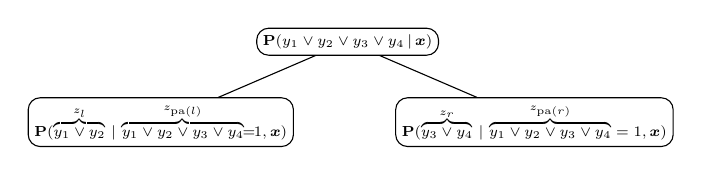
\begin{tikzpicture}[scale = 0.75,every node/.style={scale=0.75},
		regnode/.style={circle,draw,minimum width=1.5ex,inner sep=0pt},
		leaf/.style={circle,fill=black,draw,minimum width=1.5ex,inner sep=0pt},
		pleaf/.style={rectangle,rounded corners=1ex,draw,font=\scriptsize,inner sep=3pt},
		pnode/.style={rectangle,rounded corners=1ex,draw,font=\scriptsize,inner sep=3pt},
		rootnode/.style={rectangle,rounded corners=1ex,draw,font=\scriptsize,inner sep=3pt},
		activerootnode/.style={rectangle,rounded corners=1ex,draw,font=\scriptsize,inner sep=3pt,line width=1pt},
		activenode/.style={rectangle,rounded corners=1ex,draw,font=\scriptsize,inner sep=3pt,line width=1pt},
		activepleaf/.style={rectangle,rounded corners=1ex,draw,font=\scriptsize,inner sep=3pt,line width=1pt},
		level/.style={sibling distance=18em/#1, level distance=9ex}
		]
		\node (z) [rootnode] {\thickmuskip=-1.5mu $\prob(y_1\lor y_2 \lor y_3 \lor y_4 \given\bx)$}
		child {node (a) [pnode] {\thickmuskip=-1.5mu $\prob(\overbrace{y_1 \lor y_2}^{z_l}\given \overbrace{y_1 \lor y_2 \lor y_3  \lor y_4}^{z_{\mathrm{pa}(l)}}=1, \bx)$} 
			%child {node [label=below:{$y_1$}] (b) [pleaf,fill=lightgray] {\thickmuskip=-1.5mu $\prob(y_1\given y_1 \lor y_2=1, \bx)$} edge from parent node[above left]{}}
			%child {node [label=below:{$y_2$}] (g) [pleaf] {\thickmuskip=-1.5mu $\prob(y_2\given y_1 \lor y_2 = 1, \bx)$} edge from parent node[above right]{}}
			edge from parent node[above left]{}
		}
		child {node (j) [pnode] {$\prob(\overbrace{y_3 \lor y_4}^{z_r} \given \overbrace{y_1 \lor y_2 \lor y_3 \lor y_4}^{z_{\mathrm{pa}(r)}} = 1, \bx)$}
		%	child {node [label=below:{$y_3$}] (k) [pleaf] {\thickmuskip=-1.5mu $\prob(y_3\given y_3 \lor y_4 = 1, \bx)$} edge from parent node[above left]{}}
		%	child {node [label=below:{$y_4$}] (l) [pleaf] {\thickmuskip=-1.5mu $\prob(y_4\given y_3 \lor y_4 = 1,  \bx)$}
		%		{
		%			child [grow=right] {node (s) {} edge from parent[draw=none]
		%				child [grow=up] {node (t) {} edge from parent[draw=none]
		%					child [grow=up] {node (u) {} edge from parent[draw=none]}
		%				}
		%			}
		%		}
		%		edge from parent node[above right]{}
		%	}
			edge from parent node[above right]{}
		};
		\end{tikzpicture}
\caption{PLTs generalizes HSM}
\end{figure}


It can be easily shown that PLTs are consistent for any multi-label probability distribution $\prob$ (including the multi-class distributions).  

This is not a case of the pick-one-label heuristic used for HSM. This heuristics maps the multi-label distribution to a multi-class distribution in the following way:\footnote{We use the same notation for the probability of the $i$-th label in the multi-class distribution as the marginal probability of the multi-label distribution, since the multi-class distribution can be also coded by vectors $\by$, but with a constraint that one and only one label is active}
$$
\eta'(\bx, j) = \prob'(y_j = 1 \given \bx) = \sum_{\by \in \calY} y_j \frac{\prob(\by \given \bx)}{\sum_{j'=1}^m y_{j'}}
$$
This is specific marginalization with respect to $y_j$ in which we divide the conditional probability of  $\prob(\by \given \bx)$ by the number of ones in $\by$. To see that the pick-one-label does not lead to optimal solution let us consider a following conditional distribution for some $\bx$ given in the table below.
\begin{center}
\begin{tabular}{c c}
\toprule
labels $\by$ & probability $\prob(\by \given \bx)$ \\
\midrule
$\{1\}$ & 0.15 \\
$\{2\}$ & 0.1 \\
$\{1, 2\}$ & 0.25 \\
$\{3\}$ & 0.3 \\
$\{4\}$ & 0.2 \\
\bottomrule
\end{tabular}
\end{center}
The optimal top 1 prediction for this example is obviously label $1$, since the marginal probabilities are $\eta(\bx,1) = 0.4, \eta(\bx,2) = 0.35,  \eta(\bx,3) = 0.3, \eta(\bx,4) =0.2$. However, the pick-one-label heuristic will transform the original distribution to the following one: $\eta'(\bx,1) = 0.275, \eta'(\bx,2) = 0.225,  \eta'(\bx,3) = 0.3, \eta'(\bx,4) =0.2$. The predicted top label will be then label $3$, giving the regret of 0.1. 

%splits the probability of labels $\{1,2\}$ to half probabilities of $\{1\}$ and $\{2\}$ yielding the following marginal probabilities: $\eta(\bx,1) = 0.275, \eta(\bx,2) = 0.225,  \eta(\bx,3) = 0.3, \eta(\bx,4) =0.2$. 

It is obvious that the heuristic will change the marginal probabilities of labels (unless the distribution is multi-class), therefore in general, it will lead to inconsistent solution in terms of logistic loss. 
Interestingly, if the labels are conditionally independent, i.e.,:
$$
\prob(\by \given \bx) = \prod_{j=1}^m \prob(y_i \given \bx)\,,
$$
the optimal solution in terms of precision@k does not change. To show this let us observe the following.
Let $y_i$ and $y_j$ be so that $\prob(y_i = 1 \given \bx) \ge \prob(y_j = 1 \given \bx) $. Then in the summation over of $\by$s, we are interested in four different subsets of $\calY$: 
$$
S_{i,j}^{u,w}  =  \{\by\in \calY: y_i = u \land y_j = w\} \quad u,w \in \{0,1\} \,.
$$
During mapping any $\by \in S^{0,0}_{i,j}$ does not play any role. For each $\by \in S^{1,1}_{i,j}$, the value of $y_t \frac{\prob(\by \given \bx)}{\sum_{t'=1}^m y_{t'}}$ is the same for both $y_i$ and $y_j$. Now, let $\by' \in S^{1,0}_{i,j}$ and $\by'' \in S^{0,1}_{i,j}$ be the same on all elements except the $i$-th and the $j$-th one. Then, because   $\prob(y_i = 1 \given \bx) \ge \prob(y_j = 1 \given \bx) $, we will have $\prob(\by' \given \bx) \ge \prob(\by'' \given \bx)$. Therefore, after mapping we will get $\eta'(\bx,i) \ge \eta'(\bx, j)$. 

%0.1 0.2
%0    0    0.72
%0    1    0.18
%1    0    0.08
%1    1    0.02
%
%
%0.09 0.019
%
%0.1 0.5
%0    0    0.45
%0    1    0.45
%1    0    0.05
%1    1    0.05

%0.075 0.475



\vspace{\sectionBefore}
\section{PLTs for document tagging}
\label{sec:tagging_PLTs}
\vspace{\sectionAfter}


PLTs can be combined with various underlying document representations. In this section we briefly describe sample applications of PLTs to document tagging. 
The described approaches differ mainly in the representation of a document, and therefore in the architecture of the entire model. In principle PLTs work the same in each of them, however in certain cases the application must be suited for the architecture.

All the examples consist of two modules: text representation and tagging, as presented on the schema on Figure~\ref{pic:module-repres-module-tag}. The text representation module $f : \calW^{n} \rightarrow \R^{d \times n}$ is a (not necessarily) parametric function whose input is a document and its output is the vector representation of the document. The dimension of the representation space is $d$. 
The input of the tagging input is the output of the text representation module, that is $g: \R^{d \times n} \rightarrow  \{ 0 , 1 \}^m$. 

\begin{figure}
	\begin{center}
		
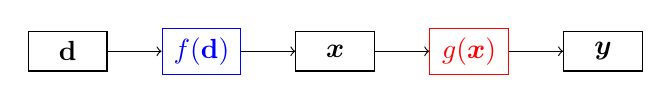
\begin{tikzpicture}[block/.style = {rectangle, draw, minimum height=0.5cm, minimum width=1cm}
]
%,yshift=0.5cm


\node (layerinput)[block]{$\mathbf{d}$};
\node (layerrepresentation)[block,right of=layerinput, xshift=.7cm, blue]{$f(\mathbf{d})$};
\node (x)[block,right of=layerrepresentation, xshift=.7cm]{$\bx$};
\node (layertagger)[block,right of=x, xshift=.7cm, red]{$g(\bx)$};
\node (layeroutput)[block,right of=layertagger, xshift=.7cm]{$\by$};

%\draw [red, thick, aligned dash] (-3.75,0.48) rectangle (3.75,-1.5);

\draw[->] ($(layerinput.north east)!0.5!(layerinput.south east)$) -- node[below] {} ($(layerrepresentation.north west)!0.5!(layerrepresentation.south west)$);
\draw[->] ($(layerrepresentation.north east)!0.5!(layerrepresentation.south east)$) -- node[above]{} ($(x.north west)!0.5!(x.south west)$);
\draw[->] ($(x.north east)!0.5!(x.south east)$) -- node[above]{} ($(layertagger.north west)!0.5!(layertagger.south west)$);
\draw[->] ($(layertagger.north east)!0.5!(layertagger.south east)$) -- node[below] {} ($(layeroutput.north west)!0.5!(layeroutput.south west)$);

\end{tikzpicture}
%\end{document}
	\end{center}
	\caption{A schema of all the described models.}
	\label{pic:module-repres-module-tag}
\end{figure}


\vspace{\sectionBefore}
\subsection{Online training of PLTs}
\label{sec:online_PLTs}
\vspace{\sectionAfter}

PLTs can be trained by using online algorithms such as different variants of stochastic gradient descent~\citep{Bottou_2010}. This is because each node can be trained in isolation (there is no dependence between node classifiers). Since the goal is to train a model for estimating probabilities $\heta_T(\bx,j)$, one can use any algorithm that minimizes log and squared error loss. By appropriate assignment of training examples to nodes (as in Algorithm~\ref{alg:plt-training}) we can easily observe that the node classifiers can be updated in online manner. 
This is important as in case of text classification problems we usually deal with data sets of a large number of examples (i.e., text documents). Moreover, a PLT can also be easily used as the last layer in a deep or shallow neural network. 

%To apply PLTs to large data and neural networks an online training algorithm is necessary.
%The online training algorithm for PLTs is given in Algorithm \ref{algo:plt-train}. 
%Let $(\bx, \by)$ be a training example. The online update of a PLT requires finding the sum, denoted with  $N_{path}$, of the sets of nodes on $\Path{y_i}$ for all $y_i \in \mathcal{P}(\by)$. The set of neighbors of nodes in $N_{path}$ that are not in $N_{path}$ is denoted with $N_{\lnot path}$. All nodes in $N_{path}$ are updated with $(\bx, 1)$, and all the nodes in $N_{\lnot path}$ with $(\bx, 0)$. The described learning algorithm can be applied to many different underlying models for document representation. 
%%
\begin{algorithm}[]
	\caption{Incremental learning of a \Algo{PLT}}
	\label{algo:plt-train}
	\begin{algorithmic}[1]
	\State \textbf{input:} a label tree $T$, an online learning algorithm $A_{\textrm{online}}$, and a training set $\mathcal{S}$
	\State \textbf{output:} a set of probability estimation classifiers $\mathcal{G}$
	\State $\mathcal{G} = \emptyset$
	\For{each node $t \in T$} 
	\State $\heta_T(\cdot,t) = \textsc{nc}()$  
	\State  $\mathcal{G} = \mathcal{G} \cup \heta_T(\cdot,t) $  
	\EndFor
	
	\For{each instance $(\bx, \by) \in \mathcal{S}$}
	
	\If{$|\mathcal{P}(\by) = 0$}
	\State $N_{\textrm{path}} = \emptyset$
	\State ${N}_{\lnot \textrm{path}} = \{r_T\}$
	\Else
	
	\State $N_{\textrm{leaf}} = \{\leaf{\ell_i} : \ell_i \in \mathcal{P}(\by)\}$
	\State $N_{\textrm{path}} = \bigcup\limits_{i \in {N}_{\textrm{leaf}} } \Path{i}$
	%\State ${N}_{\lnot path} = \textsc{Neighbors}({N}_{path})$ \Comment{a set of neighbor nodes of ${N}$ that are not in ${N}$}
	\State ${N}_{\lnot \textrm{path}} = \{t \in T: \exists_{t' \in N_{\textrm{path}}} \pa{t} = \pa{t'}\} \setminus N_{\textrm{path}}$

	\EndIf
	
	\For{$t \in \mathcal{N}_{\textrm{path}}$}
	$\heta_T(\cdot,t) = A_{\textrm{online}}(\heta_T, \bx, 1)$
	\EndFor
	
	\For{$t \in \mathcal{N}_{\lnot \textrm{path}}$}
	$\heta_T(\cdot,t) = A_{\textrm{online}}(\heta_T, \bx, 0)$
	\EndFor
	
	\EndFor		
	\State \textbf{return} a set of probability estimation classifiers $\mathcal{H}$. 
\end{algorithmic}

\end{algorithm}


\vspace{\sectionBefore}
\subsection{PLTs with sparse input}
\label{sec:sparse_input}
\vspace{\sectionAfter}

In the simplest case PLTs can be used on sparse representation of text. In other words, the text representation module $f$ can transform text to bag-of-words representation, in which case $d=N$. However, on average the number of non-zero features $\overline{\mathrm{nnz}}(\bx) \ll N$, and the documents are represented as sparse matrices. %The training is a direct application of the training Algorithm \ref{algo:plt-train}.
There are two possibilities how to work with the sparse representation. When batch training is feasible, one can train the models effectively one by one, or in parallel, in a dense format, and then store them in a sparse format. However, when online training is required, it is necessary use of feature hashing~\citep{Weinberger_et_al_2009} to make the memory requirements feasible. 

Interestingly, in the case of sparse features, the space complexity can be significantly reduced as well. Admittedly, the number of models is the highest for binary trees and can be as high as $2m-1$ (notice that the size of a tree with $m$ leaves is upper bounded by $2m-1$). This is twice the number of models in the simplest 1-vs-all approach. Paradoxically, the space complexity can be the lowest at this upper bound. This is because only the sibling nodes need to share the same features, while no other features are needed to build corresponding classifiers. Therefore, only those (few) features needed to describe the sibling labels have to be used in the models. If the space complexity still exceeds the available memory, one can always use feature hashing over all nodes \cite{Weinberger_et_al_2009}.


\vspace{\sectionBefore}
\subsection{PLTs with word embeddings}
\label{sec:sparse_input}
\vspace{\sectionAfter}

Instead of the sparse representation we can also use a dense representation being a result of a deep or shallow neural network.
One possibility is to use pretrained word embeddings, like word2vec~\citep{word2vec} or glove~\citep{glove}. This idea is presented on Figure~\ref{pic:model-embedding}. The document representation can be created from the word representations in many ways, i.e, as an average \cite{!} or as the maximum or minimum value of each element \cite{!}.

It is possible to train the word embeddings simultaneously with the tagger module, similarly as in FastText~\citep{}. Depending on the application and the size of the text corpus this might be either inferior or superior to the former approach. Another option is to initiate the network with the pre-trained values and then update all the parameters of both the tagging and text representation module. 
%but such approach leads to serious lengthening of the training time \cite{!!} and often to worse results\cite{!!}. This is not surprising since the pretrained word embeddings represent knowledge transfered from larger text corpora then the tagging datasets.

\begin{figure}
	\begin{center}
		
%\usepackage{tikz}
%\usetikzlibrary{positioning,calc}
%  \tikzset{}
%  }

\makeatletter
\def\pgf@dec@dashon{5pt}
\def\pgf@dec@dashoff{5pt}
\pgfkeys{/pgf/decoration/.cd,
	dash on/.store in=\pgf@dec@dashon,
	dash off/.store in=\pgf@dec@dashoff
}
\pgfdeclaredecoration{aligned dash}{start}{
	\state{start}[width=0pt, next state=pre-corner,persistent precomputation={
		\pgfextract@process\pgffirstpoint{\pgfpointdecoratedinputsegmentfirst}%
		\pgfextract@process\pgfsecondpoint{\pgfpointdecoratedinputsegmentlast}%
		\pgfmathsetlengthmacro\pgf@dec@dashon{\pgf@dec@dashon}%
		\pgfmathsetlengthmacro\pgf@dec@dashoff{\pgf@dec@dashoff}%
		\pgfmathsetlengthmacro\pgf@dec@halfdash{\pgf@dec@dashon/2}%
	}]{}
	\state{pre-corner}[width=\pgfdecoratedinputsegmentlength, next state=post-corner, persistent precomputation={
		%
		\pgfmathparse{int(ceil((\pgfdecoratedinputsegmentlength-\pgf@dec@dashon-\pgf@dec@dashoff)/(\pgf@dec@dashon+\pgf@dec@dashoff)))}%
		\let\pgf@n=\pgfmathresult
		\pgfmathsetlengthmacro\pgf@b%
		{\pgfdecoratedinputsegmentlength/(\pgf@n+1)-\pgf@dec@dashon}%
		\ifdim\pgf@b<\pgf@dec@dashoff\relax%
		\pgfmathparse{int(\pgf@n-1)}\let\pgf@n=\pgfmathresult%
		\pgfmathsetlengthmacro\pgf@b%
		{\pgfdecoratedinputsegmentlength/(\pgf@n+1)-\pgf@dec@dashon}%
		\fi%
		\pgfmathsetlengthmacro\pgf@b{\pgf@b+\pgf@dec@dashon}%
	}]{%
	\pgfmathloop
	\ifnum\pgfmathcounter>\pgf@n%
	\else%
	\pgfpathmoveto{\pgfpoint{\pgf@b*\pgfmathcounter-\pgf@dec@halfdash}{0pt}}%
	\pgfpathlineto{\pgfpoint{\pgf@b*\pgfmathcounter+\pgf@dec@halfdash}{0pt}}%
	\repeatpgfmathloop%
	\pgfpathmoveto%
	{\pgfpoint{\pgfdecoratedinputsegmentlength-\pgf@dec@halfdash}{0pt}}%
	\pgfpathlineto%
	{\pgfpointdecoratedinputsegmentlast}
}
\state{post-corner}[width=0pt, next state=pre-corner]{
	\pgfpathlineto{\pgfpoint{\pgf@dec@halfdash}{0pt}}%
}
\state{final}{
	\pgftransformreset%
	\pgfpathlineto{\pgfpointlineatdistance{\pgf@dec@halfdash}{\pgffirstpoint}{\pgfsecondpoint}}%
}
}
\tikzset{aligned dash/.style={
		decoration={aligned dash, #1}, decorate
	}}
	
	\begin{tikzpicture}[layer/.style = {rectangle, draw, minimum height=0.5cm, minimum width=7cm},
	xinput/.style = {rectangle, draw, minimum height=0.5cm, minimum width=1cm},
	dotsinput/.style = {rectangle, minimum height=0.5cm, minimum width=1cm},
	]
	%,yshift=0.5cm
	
	
	\node (layerembedding)[layer]{word embeddings};
	\node (layeragregation)[layer,above of=layerembedding]{$\bx$};
	\node (layertagger)[layer,above of=layeragregation]{PLT};
	\node (layeroutput)[layer,above of=layertagger]{output};
	
	\node (x1)[xinput,below of=layerembedding, xshift=-3cm]{$w_1$};
	\node (x2)[xinput,below of=layerembedding, xshift=-1.5cm]{$w_2$};
	\node (xdots)[dotsinput,below of=layerembedding, xshift=0cm]{\ldots};
	\node (x3)[xinput,below of=layerembedding, xshift=1.5cm]{$w_{n-1}$};
	\node (x4)[xinput,below of=layerembedding, xshift=3cm]{$w_{n}$};
	
	\draw [red, thick, aligned dash] (-3.75,3.5) rectangle (3.75,1.52);
	\draw [blue, thick, aligned dash] (-3.75,1.48) rectangle (3.75,-1.5);
	
	\draw[->] ($(layerembedding.north west)!0.5!(layerembedding.north east)$) -- node[below] {} ($(layeragregation.south west)!0.5!(layeragregation.south east)$);
	\draw[->] ($(layeragregation.north west)!0.5!(layeragregation.north east)$) -- node[below] {} ($(layertagger.south west)!0.5!(layertagger.south east)$);
	\draw[->] ($(layertagger.north west)!0.5!(layertagger.north east)$) -- node[below] {} ($(layeroutput.south west)!0.5!(layeroutput.south east)$);
	
	
	\draw[->] ($(x1.north west)!0.50!(x1.north east)$) -- node[below] {} ($(layerembedding.south west)!0.07142857142!(layerembedding.south east)$);
	
	
	\draw[->] ($(x2.north west)!0.50!(x2.north east)$) -- node[below] {} ($(layerembedding.south west)!0.28571428571!(layerembedding.south east)$);
	
	
	\draw[->] ($(x3.north west)!0.50!(x3.north east)$) -- node[below] {} ($(layerembedding.south west)!0.71428571428!(layerembedding.south east)$);
	
	
	\draw[->] ($(x4.north west)!0.50!(x4.north east)$) -- node[below] {} ($(layerembedding.south west)!0.92857142857!(layerembedding.south east)$);
	% more arrows here
	\end{tikzpicture}
	
	
%%\usepackage{tikz}
%%\usetikzlibrary{positioning,calc}
%%  \tikzset{}
%%  }
%
%\makeatletter
%\def\pgf@dec@dashon{5pt}
%\def\pgf@dec@dashoff{5pt}
%\pgfkeys{/pgf/decoration/.cd,
%	dash on/.store in=\pgf@dec@dashon,
%	dash off/.store in=\pgf@dec@dashoff
%}
%\pgfdeclaredecoration{aligned dash}{start}{
%	\state{start}[width=0pt, next state=pre-corner,persistent precomputation={
%		\pgfextract@process\pgffirstpoint{\pgfpointdecoratedinputsegmentfirst}%
%		\pgfextract@process\pgfsecondpoint{\pgfpointdecoratedinputsegmentlast}%
%		\pgfmathsetlengthmacro\pgf@dec@dashon{\pgf@dec@dashon}%
%		\pgfmathsetlengthmacro\pgf@dec@dashoff{\pgf@dec@dashoff}%
%		\pgfmathsetlengthmacro\pgf@dec@halfdash{\pgf@dec@dashon/2}%
%	}]{}
%	\state{pre-corner}[width=\pgfdecoratedinputsegmentlength, next state=post-corner, persistent precomputation={
%		%
%		\pgfmathparse{int(ceil((\pgfdecoratedinputsegmentlength-\pgf@dec@dashon-\pgf@dec@dashoff)/(\pgf@dec@dashon+\pgf@dec@dashoff)))}%
%		\let\pgf@n=\pgfmathresult
%		\pgfmathsetlengthmacro\pgf@b%
%		{\pgfdecoratedinputsegmentlength/(\pgf@n+1)-\pgf@dec@dashon}%
%		\ifdim\pgf@b<\pgf@dec@dashoff\relax%
%		\pgfmathparse{int(\pgf@n-1)}\let\pgf@n=\pgfmathresult%
%		\pgfmathsetlengthmacro\pgf@b%
%		{\pgfdecoratedinputsegmentlength/(\pgf@n+1)-\pgf@dec@dashon}%
%		\fi%
%		\pgfmathsetlengthmacro\pgf@b{\pgf@b+\pgf@dec@dashon}%
%	}]{%
%	\pgfmathloop
%	\ifnum\pgfmathcounter>\pgf@n%
%	\else%
%	\pgfpathmoveto{\pgfpoint{\pgf@b*\pgfmathcounter-\pgf@dec@halfdash}{0pt}}%
%	\pgfpathlineto{\pgfpoint{\pgf@b*\pgfmathcounter+\pgf@dec@halfdash}{0pt}}%
%	\repeatpgfmathloop%
%	\pgfpathmoveto%
%	{\pgfpoint{\pgfdecoratedinputsegmentlength-\pgf@dec@halfdash}{0pt}}%
%	\pgfpathlineto%
%	{\pgfpointdecoratedinputsegmentlast}
%}
%\state{post-corner}[width=0pt, next state=pre-corner]{
%	\pgfpathlineto{\pgfpoint{\pgf@dec@halfdash}{0pt}}%
%}
%\state{final}{
%	\pgftransformreset%
%	\pgfpathlineto{\pgfpointlineatdistance{\pgf@dec@halfdash}{\pgffirstpoint}{\pgfsecondpoint}}%
%}
%}
%\tikzset{aligned dash/.style={
%		decoration={aligned dash, #1}, decorate
%	}}
%	
%\begin{tikzpicture}[layer/.style = {rectangle, draw, minimum height=0.5cm, minimum width=7cm},
%xinput/.style = {rectangle, draw, minimum height=0.5cm, minimum width=1cm},
%]
%        %,yshift=0.5cm
%        
%        
%    \node (layerembedding)[layer]{word embeddings};
%    \node (layertagger)[layer,above of=layerembedding]{PLT};
%    \node (layeroutput)[layer,above of=layertagger]{output};
%    
%    \node (x1)[xinput,below of=layerembedding, xshift=-3cm]{$x_1$};
%    \node (x2)[xinput,below of=layerembedding, xshift=-1.5cm]{$x_2$};
%    \node (x3)[xinput,below of=layerembedding, xshift=1.5cm]{$x_{d-1}$};
%    \node (x4)[xinput,below of=layerembedding, xshift=3cm]{$x_{d}$};
%    
%    \draw [blue, thick, aligned dash] (-3.75,2.5) rectangle (3.75,0.52);
%    \draw [red, thick, aligned dash] (-3.75,0.48) rectangle (3.75,-1.5);
%    
%    \draw[->] ($(layerembedding.north west)!0.5!(layerembedding.north east)$) -- node[below] {} ($(layertagger.south west)!0.5!(layertagger.south east)$);
%    \draw[->] ($(layertagger.north west)!0.5!(layertagger.north east)$) -- node[below] {} ($(layeroutput.south west)!0.5!(layeroutput.south east)$);
%    
%    
%    \draw[->] ($(x1.north west)!0.50!(x1.north east)$) -- node[below] {} ($(layerembedding.south west)!0.07142857142!(layerembedding.south east)$);
%    
%    
%    \draw[->] ($(x2.north west)!0.50!(x2.north east)$) -- node[below] {} ($(layerembedding.south west)!0.28571428571!(layerembedding.south east)$);
%    
%    
%    \draw[->] ($(x3.north west)!0.50!(x3.north east)$) -- node[below] {} ($(layerembedding.south west)!0.71428571428!(layerembedding.south east)$);
%    
%    
%    \draw[->] ($(x4.north west)!0.50!(x4.north east)$) -- node[below] {} ($(layerembedding.south west)!0.92857142857!(layerembedding.south east)$);
%    % more arrows here
%\end{tikzpicture}
%%\end{document}
	\end{center}
	\caption{PLT with word embedding.}
	\label{pic:model-embedding}
\end{figure}


%\vspace{\sectionBefore}
%\subsection{PLTs with recurrent neural network}
%\label{sec:sparse_input}
%\vspace{\sectionAfter}

\vspace{\sectionBefore}
\subsection{PLTs with LSTM}
\label{sec:sparse_input}
\vspace{\sectionAfter}

To improve the document representation, instead of a simple average over words, we feed the embeddings of consecutive words into an LSTM newtork~\citep{!}. The output of the LSTM is then input of the tagger.

\vspace{\sectionBefore}
\section{Empirical results}
\label{sec:empirical_results}
\vspace{\sectionAfter}


\subsection{Comparison of PLTs and HSM on synthetic data}
\label{sec:empirical-synthetic}

To validate the theoretical results we perform a comparison of PLTs and HSM on synthetic datasets of three types: multi-label with conditionally dependent labels, multi-label with independent labels, and multi-class. The empirical results are given in Table \ref{tab:synthetic1}. The methods used to generate the data are given below.

The independent multi-label data was generated from a multi-label OvR model. Example features $\bx$ were generated by uniformly drawing from $[-0.5, 0.5]^d$. The OvR weights $W$ were drawn uniformly from  $[-0.5, 0.5]^{d \times m}$.
%, where $s$ stands for a shift used to control the average probability of a positive label. 
The score $a =\bx w_i$ of $i$-th label was then transformed to a probability $p_i(a) = \frac{1}{(1 + exp(-a))}$, and the $i$-th label was drawn with the probability $p_i$.

% The conditionally dependent multi-label data was generated from the PCC \cite{!} model. Example features were drawn as in the previous paragraph. The PCC model weights were drawn from  $[-0.5, 0.5]^{(d + m) \times m}$.
% %, also with the use of a shift $s$. 
% The score of $i$-th label was computed based on it's features and all the previous labels $j$ as $d+j$-th features, set to -$q$ or $q$ depending on the results of the draws with labels probabilities. The value of $q$, usually set to $0.5$, is related to the degree of dependence between labels.


The conditionally dependent multi-label data was generated according to the following model:
\begin{equation*}
\boldsymbol{f} = \boldsymbol{A }\bx + \epsilon 
\end{equation*}
\begin{equation*}
\by = \assert{\boldsymbol{M} \boldsymbol{f} >  0  },
\end{equation*}

\noindent
where $\boldsymbol{f} = (f_1, f_2, \ldots, f_m)$ represent $m$ latent variables, $\boldsymbol{M}$ a mixing matrix, and $\epsilon$ a noise introducing label dependencies. The two-dimensional feature vector $\bx$ was drawn uniformly from a unit disc, the linear coefficients $A$ uniformly from two-dimensional unit sphere. The noise $\epsilon$ is a $m$-dimensional vector drawn from $N(0, 0.25)$, and the $m \times m$ mixing matrix $\boldsymbol{m}$ i.i.d. from $[-1, 1]$. To make the labels dependent $\boldsymbol{M} \neq \boldsymbol{I}$.

The multi-class data was generated based on the same model as independent multi-label data, OvR, but we selected the label with the highest probability, instead of drawing $m$ times. 

\textbf{TODO: this table will contain some other results}

\begin{table}[]
	\centering
	\caption{Precision@1 of PLT and HSM on synthetic data. The number of passes gives the number of epochs of training. The values of precision@1 are averages of 10 random runs.}
	\label{tab:synthetic1}
\begin{tabular}{l|rr|rr|rr}
	\toprule
	 & \multicolumn{2}{c|}{dependent}                     & \multicolumn{2}{c|}{independent}                   & \multicolumn{2}{c}{multiclass}                    \\
	 passes & \multicolumn{1}{c}{PLT} & \multicolumn{1}{c|}{HSM} & \multicolumn{1}{c}{PLT} & \multicolumn{1}{c|}{HSM} & \multicolumn{1}{c}{PLT} & \multicolumn{1}{c}{HSM} \\
	\midrule
	1      & 73.17 & 72.04 & 61.87    & 53.64 & 34.31  & 34.31  \\
	10     & 85.51 & 84.16 & 63.36    & 58.00 & 38.67  & 38.67  \\
	100    & 89.09 & 85.48 & 62.23    & 60.45 & 36.71  & 36.71  \\
	1000   & 87.12 & 84.76 & 62.69    & 61.98 & 34.26  & 34.26 \\
	\bottomrule
\end{tabular}
\end{table}


\newpage



\bibliography{xmlc_references}
\bibliographystyle{icml2018}

\appendix

\onecolumn

\section{Regret for Prec@k}


Precision@k is formally defined as:
\begin{equation}
\mathrm{precision}@k(\by, \bx, \bh) = \frac{1}{k} \sum_{j \in \calY_k} \assert{y_j = 1},
\label{eqn:precision-at-k}
\end{equation}
where $\calY_k$ is a set of $k$ labels predicted by $\bh$ for $\bx$.
%
The loss function for precision$@k$ is $\ell_{p@k} = 1 - \mathrm{precision}@k$. The conditional risk for this loss is given by:
\begin{eqnarray*}
\loss_{P@k}(\bh \given \bx) & = & \mathbb{E} \ell_{p@k}(\by,\bx, \bh) \\
& = & 1 - \sum_{\by \in \calY} \Pr(\by \given \bx) \frac{1}{k} \sum_{j \in \calY_k} \assert{y_j = 1} \\
& = & 1 - \frac{1}{k} \sum_{j \in \calY_k} \sum_{\by \in \calY} \Pr(\by \given \bx) \assert{y_j = 1} \\
& = & 1 - \frac{1}{k} \sum_{j \in \calY_k} \eta(\bx,j) \,.
\end{eqnarray*}
%
The above result shows that the optimal strategy for precision$@k$ is to predict $k$ labels
with the highest conditional probabilities $\eta(\bx,j)$.


Top-k labels with respect to the true marginals
\[
M_k(\bx) = \left\{ i\in [m] : \# \left\{ j \in [m] : \eta(\bx, j) \ge \eta(\bx, i)  \right\} \le k\right\}
\]

Top-k labels with respect to the estimated marginals
\[
\hat{M}_k(\bx) = \left\{ i\in [m] : \# \left\{ j \in [m] : \hat{\eta}(\bx, j) \ge \hat{\eta}(\bx, i)  \right\} \le k\right\}
\]


Expected regret for Prec@k conditioned on $\bx$ 
\[
\mbox{Reg}_{P@k} (h, \bx) = \sum_{i \in M_k(\bx)} \eta (\bx ,i ) - \sum_{j \in [m]} h(\bx, j) \eta(\bx , j )
\]

We shall focus on multi-label classifiers in the following form:
\[
h(\bx,i) =h_{k, \hat{\eta}}(\bx,i) = \assert{\textstyle i \in \hat{M}_k(\bx) }
\]

In this case the Prec@k regret is $[0,1]$.

The error for marginal estimates is denoted by $m_i = \vert \eta (\bx ,i ) - \hat{\eta} (\bx ,i )\vert$. With this we can upper bound 
\begin{align}
\mbox{Reg}_{P@k} (h, \bx) 
  & = \sum_{i \in M_k(\bx)} \eta (\bx ,i ) - \sum_{j \in [m]} h(\bx, j) \eta(\bx , j ) \notag \\
  & \le \sum_{i \in M_k(\bx)} \hat{\eta} (\bx ,i ) + m_i - \sum_{j \in [m]} h(\bx, j) \eta(\bx , j ) \notag \\ 
  & \le \sum_{i \in \hat{M}_k(\bx)} (\hat{\eta} (\bx ,i ) + m_i )- \sum_{j \in \hat{M}_k(\bx)}  \eta(\bx , j ) \notag \\
  & = \sum_{i \in \hat{M}_k(\bx)} 2m_i \notag \\
  & \le 2k\max_{i \in [m]} m_i
\end{align}

\section{Probabilistic label trees}
\label{app:plt}

An example of a probabilistic label tree (\Algo{PLT}) for 4 labels $(y_1,y_2,y_3,y_4)$ is given in Fig.~\ref{fig:plt}. To estimate posterior probability $\eta(\bx, j) = \prob(y_j = 1 \given \bx)$, \Algo{PLT} uses a path from a root to the $j$-th leaf.
In each node $t$, we associate with a training instance $(\bx,\by)$ a label $z_t$ such that:
$$
z_t = \assert{\textstyle \sum_{j \in L(t)} y_j \ge 1} \quad \textrm{(or equivalently $z_t = \bigvee_{j \in L(t)} y_j$)}
$$
Recall that $L(t)$ is a set of all leaves of a subtree with the root in the $t$-th node. In leaf nodes the labels $z_j$, $j \in L$, correspond to original labels $y_j$.
%
\begin{figure}[h]
	\begin{center}
		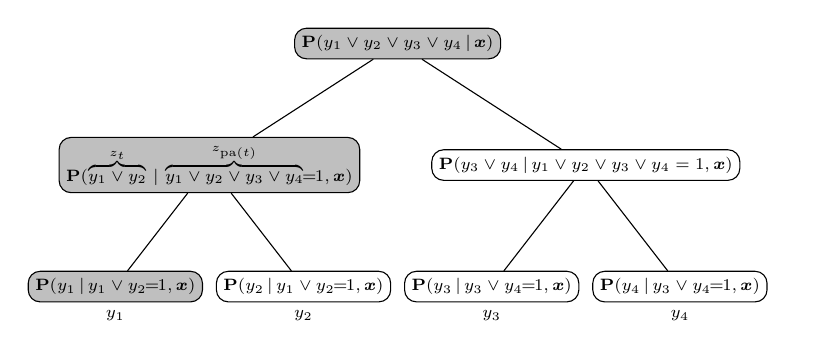
\begin{tikzpicture}[scale = 0.85,every node/.style={scale=0.85},
		regnode/.style={circle,draw,minimum width=1.5ex,inner sep=0pt},
		leaf/.style={circle,fill=black,draw,minimum width=1.5ex,inner sep=0pt},
		pleaf/.style={rectangle,rounded corners=1ex,draw,font=\scriptsize,inner sep=3pt},
		pnode/.style={rectangle,rounded corners=1ex,draw,font=\scriptsize,inner sep=3pt},
		rootnode/.style={rectangle,rounded corners=1ex,draw,font=\scriptsize,inner sep=3pt},
		activerootnode/.style={rectangle,rounded corners=1ex,draw,font=\scriptsize,inner sep=3pt,line width=1pt},
		activenode/.style={rectangle,rounded corners=1ex,draw,font=\scriptsize,inner sep=3pt,line width=1pt},
		activepleaf/.style={rectangle,rounded corners=1ex,draw,font=\scriptsize,inner sep=3pt,line width=1pt},
		level/.style={sibling distance=16em/#1, level distance=12ex}
		]
		\node (z) [rootnode,fill=lightgray] {\thickmuskip=-1.5mu $\prob(y_1\lor y_2 \lor y_3 \lor y_4 \given\bx)$}
		child {node (a) [pnode,fill=lightgray] {\thickmuskip=-1.5mu $\prob(\overbrace{y_1 \lor y_2}^{z_t}\given \overbrace{y_1 \lor y_2 \lor y_3  \lor y_4}^{z_{\mathrm{pa}(t)}}=1, \bx)$} 
			child {node [label=below:{ \scriptsize \thickmuskip=-1.5mu $y_1$}] (b) [pleaf,fill=lightgray] {\thickmuskip=-1.5mu $\prob(y_1\given y_1 \lor y_2=1, \bx)$} edge from parent node[above left]{}}
			child {node [label=below:{\scriptsize \thickmuskip=0mu $y_2$}] (g) [pleaf] {\thickmuskip=-1.5mu $\prob(y_2\given y_1 \lor y_2 = 1, \bx)$} edge from parent node[above right]{}}
			edge from parent node[above left]{}
		}
		child {node (j) [pnode] {$\prob(y_3 \lor y_4 \given y_1 \lor y_2 \lor y_3 \lor y_4 = 1, \bx)$}
			child {node [label=below:{ \scriptsize \thickmuskip=0mu $y_3$}] (k) [pleaf] {\thickmuskip=-1.5mu $\prob(y_3\given y_3 \lor y_4 = 1, \bx)$} edge from parent node[above left]{}}
			child {node [label=below:{ \scriptsize \thickmuskip=0mu $y_4$}] (l) [pleaf] {\thickmuskip=-1.5mu $\prob(y_4\given y_3 \lor y_4 = 1,  \bx)$}
				{
					child [grow=right] {node (s) {} edge from parent[draw=none]
						child [grow=up] {node (t) {} edge from parent[draw=none]
							child [grow=up] {node (u) {} edge from parent[draw=none]}
						}
					}
				}
				edge from parent node[above right]{}
			}
			edge from parent node[above right]{}
		};
		\end{tikzpicture}
\end{center}
\caption{An example of a probabilistic label tree for 4 labels $(y_1,y_2,y_3,y_4)$.}
\label{fig:plt}
\end{figure}
%

Consider the leaf node $j$ and the path from the root to this leaf node. Using the chain rule of probability, we can express $\eta(\bx, j)$ in the following way:
\begin{equation}
\eta(\bx, j) = \prod_{t \in \Path{j}} \eta_T(\bx, t)\,,
\label{eqn:probabilistic_tree_appendix}
\end{equation}
where $\eta_T(\bx, t) = \prob(z_t = 1 \given z_{\pa{t}} =1, \bx)$, for all non-root nodes $t$, and $\eta(\bx, t) = \prob(z_t = 1 \given \bx)$, if $t$ is the root node (denoted by $r(T)$). 

To see the correctness of (\ref{eqn:probabilistic_tree_appendix}) notice that $z_{t} = 1$ implies $z_{\pa{t}} = 1$. So, for non-root nodes $t$ and $\pa{t}$ we have:
\begin{eqnarray*}
\eta_T(\bx,t) \eta_T(\bx, \pa{t}) & = &  \prob(z_t = 1 \given z_{\pa{t}} =1, \bx)\prob(z_{\pa{t}} = 1 \given z_{\pa{\pa{t}}} =1, \bx)\\
& = & \frac{\prob(z_t = 1 , z_{\pa{t}} =1, \bx)}{\prob(z_{\pa{t}} =1, \bx)} \frac{\prob(z_{\pa{t}} = 1, z_{\pa{\pa{t}}} =1, \bx)}{\prob(z_{\pa{\pa{t}}} =1, \bx)} \\
& = & \frac{\prob(z_t = 1, \bx)}{\prob(z_{\pa{t}} =1, \bx)} \frac{\prob(z_{\pa{t}} = 1, \bx)}{\prob(z_{\pa{\pa{t}}} =1, \bx)} \\
& = & \frac{\prob(z_t = 1, \bx)}{\prob(z_{\pa{\pa{t}}} =1, \bx)} \,.
\end{eqnarray*}
In words, the probability associated with the parent node $\pa{t}$ cancels out and we can express $\eta_T(\bx,t) \eta_T(\bx, \pa{t})$ as the product of probabilities associated only with node $t$ and its grandparent node $\pa{\pa{t}}$. 
%
Applying the above rule consecutively to $\prod_{t \in \Path{j}} \eta_T(\bx, t)$ and recalling that for the root note $\eta_T(\bx, r(T)) = \prob(z_{r(T)} = 1 \given \bx)$, we finally get $\eta(\bx, j)$. 

Below we show that \Algo{PLT}s posses strong theoretical guarantees. We derive a relation between  estimation error minimized by the node classifiers and estimation error of posterior probabilities $\eta(\bx,j)$. This relation states that we can upperbound the latter error by the former. This also implies that for optimal node classifiers we get optimal multi-label classifier in terms of estimation of posterior probabilities.


We are interested in bounding the estimation error of posterior probabilities of labels at point $\bx$
$$
\ell(\eta(\bx),\heta(\bx)) = \frac{1}{m} \sum_{j=1}^m |\eta(\bx, j) - \heta(\bx, j)| \,,
$$
in terms of an estimation error of node classifiers
$$
\ell(\eta_T(\bx, t), \heta_T(\bx, t)) = |\eta_T(\bx, t) - \heta_T(\bx, t)  | \,.
$$

Expressing $\eta(\bx, j)$  and $\heta(\bx, j)$ by (\ref{eqn:probabilistic_tree_appendix}) and applying Lemma~2 from~\cite{Beygelzimer_et_al_2009b}, we get:
\begin{equation}
\left | \eta(\bx, j) - \heta(\bx, j) \right | \le \sum_{t \in \Path{j}} \left | \eta_T(\bx, t) - \heta_T(\bx, t) \right | \,.
\label{eqn:estimation_bound}
\end{equation}

Equation (\ref{eqn:estimation_bound}) already shows that minimization of the estimation error by node classifiers improves the overall performance of \Algo{PLT}s. We can show, however, even a more general result concerning surrogate regret bounds by referring to the theory of  strongly proper composite losses~\cite{Agarwal_2014}. 

Assume that a node classifier has a form of a real-valued function $f_t$. Moreover, there exists a strictly increasing (and therefore invertible) link function $\psi: [0,1] \rightarrow \mathbb{R}$ such that $f_t(\bx) = \psi(\heta_T(\bx,t))$. Recall that the regret of $f_t$ in terms of a loss function $\ell$ at point $\bx$ is defined as:
$$
\reg_{\ell}(f_t \given \bx) = L_{\ell}(f_t \given \bx) - L_{\ell}^*(\bx) \,,
$$
where $L_{\ell}(f_t \given \bx)$ is the expected loss  at  point $\bx$:
$$
L_{\ell}(f \given \bx) = \mathbb{E}_{y_j\given\bx} \left [ \ell  (y_j, f_t(\bx)) \right ] \,,
$$
and  $L_{\ell}^*(\bx)$ is the minimum expected loss at point $\bx$.

If a node classifier is trained by a learning algorithm that minimizes a strongly proper composite loss, e.g.,  squared, exponential, or logistic loss, like in our implementation (see in Appendix \ref{sec:training_of_node_classifiers}), then the bound (\ref{eqn:estimation_bound}) can be expressed in terms of the regret of this loss function: 
$$
\left | \eta_T(\bx, t) - \psi^{-1}(f_t)  \right | \le \sqrt{ \frac{2}{\lambda}} \sqrt{\reg_\ell(f_t \given \bx)}
$$
where $\lambda$ is a strong properness constant specific for a given loss function (for more detail, see~\cite{Agarwal_2014}). By putting the above inequality into~(\ref{eqn:estimation_bound}), we get
$$
\left | \eta(\bx, j) - \heta(\bx, j) \right | \le \! \sum_{t \in \Path{j}} \! \left | \eta_T(\bx, t) - \heta_T(\bx, t) \right | = \!  \sum_{t \in \Path{j}}  \! \left | \eta_T(\bx, t) - \psi^{-1}(f_t)  \right | \le  \! \sum_{t \in \Path{j}}  \! \sqrt{ \frac{2}{\lambda}} \sqrt{\reg_\ell(f_t \given \bx)}
$$ 


%Consider the label-wise KL-divergence between true posterior probabilities $\eta(\bx, j)$ and their estimates $\heta(\bx, j)$:
%$$
%\KLD(\eta(\bx) || \heta(\bx)) = \frac{1}{m}\sum_{j=1}^m \KLD(\eta(\bx,j) || \heta(\bx,j)) = \frac{1}{m}\sum_{j=1}^m \left ( \eta(\bx,j) \log \frac{\eta(\bx,j)}{\heta(\bx,j)} + (1 -\eta(\bx,j)) \log \frac{1- \eta(\bx,j)}{1 - \heta(\bx,j)}\right ) 
%$$
%Let us remark that $\KLD(\eta(\bx,j) || \heta(\bx,j))$  is equivalent to the conditional logistic regret defined as:
%$$
%\reglog(\heta(\bx,j) \given \bx) = L_{\log}(\heta(\bx,j) \given \bx) - L_{\log}^*(\bx) \,,
%$$
%where $L_{\log}(\heta(\bx,j) \given \bx)$ is the expected logistic risk at  point $\bx$:
%$$
%L_{\log}(\heta(\bx,j) \given \bx) = \mathbb{E}_{y_j\given\bx} \ell_{\log} (y_j, \heta(\bx,j)) = \mathbb{E}_{y_j\given\bx} \left ( y_j \log \heta(\bx,j) + (1 - y_j) \log (1 - \heta(\bx,j)) \right ) \,.
%$$
%and  $L_{\log}^*(\bx)$ is the minimum logistic risk at point $\bx$ achieved by $\heta(\bx,j) = \eta(\bx,j)$. %as says a standard result on the theory of proper losses (see, e.g., \citep{Reid_Williamson_2010}).
%
%Because of (\ref{eqn:probabilistic_tree_appendix}), we can rewrite the above to:
%$$
%\KLD(\eta || \heta) = \frac{1}{m}\sum_{j=1}^m \left (  \prod_{t \in \Path{j}} \eta_T(\bx, t)\log \frac{ \prod_{t \in \Path{j}} \eta_T(\bx, t)}{\ \prod_{t \in \Path{j}} \heta_T(\bx, t)} + (1 - \prod_{t \in \Path{j}} \eta_T(\bx, t)) \log \frac{1-  \prod_{t \in \Path{j}} \eta_T(\bx, t)}{1 -  \prod_{t \in \Path{j}} \heta_T(\bx, t)}\right ) 
%$$

\section{Training of node classifiers}
\label{sec:training_of_node_classifiers}

In each node $t$ we trained a linear classifier $f_t(\bx) = \bw \cdot \bx$, where $\bx = (1, x_1, \ldots, x_p)$.  To this end we used a variant of stochastic gradient descent to minimize logistic loss. Albeit successfully used in large scale learning, the optimization of empirical loss using stochastic gradient descent is a particularly challenging task when the number of features and labels is large. The step function should ensure a quick convergence in order to reduce the number of required training epochs. Furthermore, it should support sparse updates of the weights (i.e., only weights for non-zero features should be updated to ensure fast training time). % and auxiliary data structures. 
\citet{Duchi_Singer_2009} propose a two phase gradient step:
\begin{align*}
	\label{eq:fobos}
	\bm{w}_{t+\frac12} &= \bm{w}_t - \gamma_t \bm{g}_t\\
	\bm{w}_{t+1} &= \argmin_{\bm{w}}\left\{ \frac12 \norm[\big]{ \bm{w} - \bm{w}_{t+\frac12}}^2
	+ \lambda \gamma_{t} r(\bm{w})\right\}
\end{align*}
where $\bm{w}_t$ is the weight vector at time step $t$, $r(\bm{w})$ is a
regularization function, $\lambda$ is regularization parameter, and $\gamma_t$ is an adaptive step size, and $\bm{g}_t$ is the gradient vector at $\bm{x}_t$ of logistic loss applied to the linear model $f_t$. 

For stochastic gradient descent with $L_2^2$ regularization,
the step function reduces to
\begin{equation*}\label{eq:fobosl2}
	\bm{w}_{t+1} = \frac{\bm{w}_t - \gamma_t \bm{g}_t}{1 + \lambda\gamma_{t}}
\end{equation*}

By using  
$$
\Pi_t = \prod_{i=1}^t (1 + \lambda\gamma_{t}) 
\quad \mathrm{and} \quad \tilde{\bw}_t = \Pi_{t} \bw_t \,,
$$
we can rewrite the step function to the following form:
$$
\tilde{\bw}_{t+1}  = \tilde{\bw}_t - \Pi_{t}  \gamma_t \bm{g}_t
$$
Thanks to this transformation, we are able to make sparse updates by storing only the current value of $\Pi_t$ (one value for each node classifier). This is because the $i$-th component of $\tilde{\bw}$ does not change when $x_i$ is zero. More formally, 
$$
\tilde{w}_{i,t+1}  = \tilde{w}_{i,t} \mathrm{, if~} g_{i,t} = 0 \,.
$$
During prediction or computation of gradient $\bm{g}_t$, we use:
$$
\bw_t = \frac{\tilde{\bw}_{t}}{\Pi_{t}} \,.
$$

In our implementation we adapt the step size $\gamma_t$ as suggested in \citep{Bottou_2012}:
$$
\gamma_t = \frac{\gamma}{1 + \lambda \gamma t} \,,
$$
where $\gamma$ is an initial parameter.


\section{Tuning of hyperparameters}
\label{sec:hyper}


A \Algo{PLT} has only one global hyperparameter which is the degree of the tree denoted by $b$. The other hyperparameters are associated with the node classifiers. To tune the stochastic gradient descent described above we varied values of $\gamma$, $\lambda$, and the number of epochs. 
%
All hyperparameters were tuned by using the open-source hyperparameter optimizer \Algo{SMAC}~\cite{Hutter_et_al_2011} with a wide range of parameters, which is reported in Table \ref{tab:hyppar}. 
%We also tuned the number of epochs which is the number of times we run through the entire dataset. 
The validation process was carried out by using a $80/20$ split of the training data for every dataset we used.

\vspace{\tableBefore}
\begin{table}[ht!]
\caption{The hyperparameters of the \Algo{PLT} method and their ranges used in hyperparameter optimization,}
\label{tab:hyppar}
\begin{center}
\begin{tabular}{|c|c|c|c|c|c|c|c|}
\hline
Hyperparameter & Validation range \\%& RCV1 & AmazonCat & Wiki10 & Delicious-200K & WikiLSHTC & Amazon \\ 
\hline
$b$ & $\{2,\dots,256\}$ \\% &  $16$          & $16$      & $32$   & $2$     & &       \\ 
$\lambda$ &  $[10 - 0.000001]$ \\%& $10^{-4}$ & $10^{-4}$   & $10^{-5}$& $10^{-5}$ & &       \\ 
$\gamma$ &  $[10 - 0.000001]$ \\%& $10^{-5}$  & $10^{-5}$   & $10^{-5}$& $10^{-6}$ & &       \\ 
Num. of epochs &  $\{ 5, \dots , 30\} $ \\
\hline
\end{tabular}
\end{center}
\end{table}
\vspace{\tableAfter}




\section{F-scores by tuning the input parameters $\ba$ and $\bb$ of \Algo{OFO} algorithms}
\label{sec:OFO_a_b}

In our experimental study described in Section \ref{sec:experiments}, we did not tune the input parameter $\ba$ of the \Algo{OFO} algorithm but set all of its components to $1$. We carried out experiments for assessing the impact of the input parameter $\ba$ on the performance of \Algo{OFO}. Its optimal value was selected from the set $C = \{10000,1000,200,100,50,20,10,7,5,4,3,2\}$ based on the same validation process like in case of $\bb$ and we took into account the fact that $a_i /b_i$ should be in range $\left (\hat\pi_j / (\hat\pi_j + 1), 0.5 \right ]$, as it was pointed out in (\ref{eqn:range}). The macro F-scores computed for the test and validation set are shown in Table \ref{tab:ofo_a_b} along with the validated values of $a_i$ and $b_i$. For sake of readability, we repeat here the scores achieved by \Algo{STO} and \Algo{FTA} reported earlier in Table \ref{tab:initthreshold}. The macro F-scores achieved by \Algo{OFO} are slightly better thanks to the additional degree of freedom, and thus, the \Algo{OFO} algorithm outperforms \Algo{FTA} and \Algo{STO} algorithm on almost every datasets except the Amazon dataset in which case the \Algo{OFO} and \Algo{FTA} algorithms are tied.

%\begin{table}[ht!] 
%	\caption{The test macro F-scores obtained by validating both input parameters $a$ and $b$} 
%	\label{tab:ofo_a_b}
%	\begin{center}
%		\begin{small}
%			%\vspace{-0.1cm}
%			\begin{tabular}{l@{\hskip 3pt}| c@{\hskip 4pt} c@{\hskip 4pt} c@{\hskip 4pt} | c@{\hskip 4pt} c@{\hskip 4pt} c@{\hskip 4pt} }
%				\toprule
%Algorithm & Dataset & $a_i$ & $b_i$ & Valid. F-score & Test F-score & Test F-score  \\
%\midrule
%PLT & RCV1 & $300$ & $20000$ & $22.20$ & $22.00$ \\
%PLT & AmazonCat & $700$ & $5000$ & $33.37$ & $35.30$ \\
%PLT & wiki10 & $100$ & $200$ & $55.27$ & $30.28$ \\
%PLT & Delicious-200K & $100$ & $200$ & $34.88$ & $11.20$ \\
%PLT & WikiLSHTC & $100$ & $200$ & $39.94$ & $14.00$ \\
%PLT & Amazon & $100$ & $200$ & $54.84$ & $51.28$ \\
%\midrule
%FastXML & RCV1 & $1000$ & $100000$ & $19.84$ & $19.28$\\
%FastXML & AmazonCat & $10000$ & $100000$ & $50.21$ & $41.48$\\
%FastXML & wiki10 & $5000$ & $100000$ & $54.72$ & $29.91$\\
%FastXML & Delicious-200K & $100$ & $500$ & $35.02$ & $11.20$\\
%FastXML & WikiLSHTC & $5000$ & $100000$ & $45.78$ & $21.38$\\
%FastXML & Amazon & $10000$ & $100000$ & $53.91$ & $52.86$\\
%				\bottomrule
%			\end{tabular}
%		\end{small}
%	\end{center}
%\end{table}

\makeatletter
\setlength{\@fptop}{0pt}
\makeatother

\begin{table}[ht!] 
	\caption{The test macro F-scores obtained by validating both input parameters $a$ and $b$. The numbers in bold indicate the best score achieved on each dataset.} 
	\label{tab:ofo_a_b}
	\begin{center}
		\begin{small}
			%\vspace{-0.1cm}
			\begin{tabular}{l@{\hskip 3pt}| c@{\hskip 4pt} c@{\hskip 4pt} c@{\hskip 4pt} | c@{\hskip 4pt} c@{\hskip 4pt}  | c@{\hskip 4pt} | c@{\hskip 4pt}  }
				\toprule
		  &         &       &       &  \multicolumn{2}{c|}{\Algo{OFO}} & \Algo{FTA} & \Algo{STO} \\           	
Algorithm & Dataset & $a_i$ & $b_i$ & Valid. F-score & Test F-score & Test F-score & Test F-score  \\
\midrule
\Algo{PLT} & RCV1 & 300 & 20000 & 22.20 & { \bf 22.00 } & 20.41 & 21.16 \\
\Algo{PLT} & AmazonCat & 700 & 5000 & 33.37 & 35.30 & 34.83 & 31.64 \\
\Algo{PLT} & wiki10 & 100 & 200 & 55.27 & { \bf 30.28 } & 29.98 & 24.02 \\
\Algo{PLT} & Delicious-200K & 100 & 200 & 34.88 & {\bf 11.20} & 11.12 & 10.96 \\
\Algo{PLT} & WikiLSHTC & 100 & 200 & 39.94 & 14.00 & 12.31 & 16.22 \\
\Algo{PLT} & Amazon & 100 & 200 & 54.84 & 51.28 & 51.77 & 46.94 \\
\midrule
\Algo{FastXML} & RCV1 & 1000 & 100000 & 19.84 & 19.28 & 17.04 & 19.58 \\
\Algo{FastXML} & AmazonCat & 10000 & 100000 & 50.21 & { \bf 41.48 } & 41.07 & 37.28 \\
\Algo{FastXML} & wiki10 & 5000 & 100000 & 54.72 & 29.91 & 29.88 & 28.26 \\
\Algo{FastXML} & Delicious-200K & 100 & 500 & 35.02 & { \bf 11.20 } & 11.18 & 10.83 \\
\Algo{FastXML} & WikiLSHTC & 5000 & 100000 & 45.78 & { \bf 21.38 } & 21.24 & 20.41 \\
\Algo{FastXML} & Amazon & 10000 & 100000 & 53.91 & {\bf 52.86} & {\bf 52.86} & 47.53 \\
				\bottomrule
			\end{tabular}
		\end{small}
	\end{center}
\end{table}





\end{document} 





\section{Electronic Submission}
\label{submission}

Submission to ICML 2018 will be entirely electronic, via a web site
(not email). Information about the submission process and \LaTeX\ templates
are available on the conference web site at:
\begin{center}
\textbf{\texttt{http://icml.cc/2018/}}
\end{center}

The guidelines below will be enforced for initial submissions and
camera-ready copies. Here is a brief summary:
\begin{itemize}
\item Submissions must be in PDF\@.
\item The maximum paper length is \textbf{8 pages excluding references and
    acknowledgements, and 10 pages including references and acknowledgements}
    (pages 9 and 10 must contain only references and acknowledgements).
\item \textbf{Do not include author information or acknowledgements} in your
    initial submission.
\item Your paper should be in \textbf{10 point Times font}.
\item Make sure your PDF file only uses Type-1 fonts.
\item Place figure captions \emph{under} the figure (and omit titles from inside
    the graphic file itself). Place table captions \emph{over} the table.
\item References must include page numbers whenever possible and be as complete
    as possible. Place multiple citations in chronological order.
\item Do not alter the style template; in particular, do not compress the paper
    format by reducing the vertical spaces.
\item Keep your abstract brief and self-contained, one paragraph and roughly
    4--6 sentences. Gross violations will require correction at the
    camera-ready phase. The title should have content words capitalized.
\end{itemize}

\subsection{Submitting Papers}

\textbf{Paper Deadline:} The deadline for paper submission that is
advertised on the conference website is strict. If your full,
anonymized, submission does not reach us on time, it will not be
considered for publication. There is no separate abstract submission.

\textbf{Anonymous Submission:} ICML uses double-blind review: no identifying
author information may appear on the title page or in the paper
itself. Section~\ref{author info} gives further details.

\textbf{Simultaneous Submission:} ICML will not accept any paper which,
at the time of submission, is under review for another conference or
has already been published. This policy also applies to papers that
overlap substantially in technical content with conference papers
under review or previously published. ICML submissions must not be
submitted to other conferences during ICML's review period. Authors
may submit to ICML substantially different versions of journal papers
that are currently under review by the journal, but not yet accepted
at the time of submission. Informal publications, such as technical
reports or papers in workshop proceedings which do not appear in
print, do not fall under these restrictions.

\medskip

Authors must provide their manuscripts in \textbf{PDF} format.
Furthermore, please make sure that files contain only embedded Type-1 fonts
(e.g.,~using the program \texttt{pdffonts} in linux or using
File/DocumentProperties/Fonts in Acrobat). Other fonts (like Type-3)
might come from graphics files imported into the document.

Authors using \textbf{Word} must convert their document to PDF\@. Most
of the latest versions of Word have the facility to do this
automatically. Submissions will not be accepted in Word format or any
format other than PDF\@. Really. We're not joking. Don't send Word.

Those who use \textbf{\LaTeX} should avoid including Type-3 fonts.
Those using \texttt{latex} and \texttt{dvips} may need the following
two commands:

{\footnotesize
\begin{verbatim}
dvips -Ppdf -tletter -G0 -o paper.ps paper.dvi
ps2pdf paper.ps
\end{verbatim}}
It is a zero following the ``-G'', which tells dvips to use
the config.pdf file. Newer \TeX\ distributions don't always need this
option.

Using \texttt{pdflatex} rather than \texttt{latex}, often gives better
results. This program avoids the Type-3 font problem, and supports more
advanced features in the \texttt{microtype} package.

\textbf{Graphics files} should be a reasonable size, and included from
an appropriate format. Use vector formats (.eps/.pdf) for plots,
lossless bitmap formats (.png) for raster graphics with sharp lines, and
jpeg for photo-like images.

The style file uses the \texttt{hyperref} package to make clickable
links in documents. If this causes problems for you, add
\texttt{nohyperref} as one of the options to the \texttt{icml2018}
usepackage statement.


\subsection{Submitting Final Camera-Ready Copy}

The final versions of papers accepted for publication should follow the
same format and naming convention as initial submissions, except that
author information (names and affiliations) should be given. See
Section~\ref{final author} for formatting instructions.

The footnote, ``Preliminary work. Under review by the International
Conference on Machine Learning (ICML). Do not distribute.'' must be
modified to ``\textit{Proceedings of the
$\mathit{35}^{th}$ International Conference on Machine Learning},
Stockholm, Sweden, PMLR 80, 2018.
Copyright 2018 by the author(s).''

For those using the \textbf{\LaTeX} style file, this change (and others) is
handled automatically by simply changing
$\mathtt{\backslash usepackage\{icml2018\}}$ to
$$\mathtt{\backslash usepackage[accepted]\{icml2018\}}$$
Authors using \textbf{Word} must edit the
footnote on the first page of the document themselves.

Camera-ready copies should have the title of the paper as running head
on each page except the first one. The running title consists of a
single line centered above a horizontal rule which is $1$~point thick.
The running head should be centered, bold and in $9$~point type. The
rule should be $10$~points above the main text. For those using the
\textbf{\LaTeX} style file, the original title is automatically set as running
head using the \texttt{fancyhdr} package which is included in the ICML
2018 style file package. In case that the original title exceeds the
size restrictions, a shorter form can be supplied by using

\verb|\icmltitlerunning{...}|

just before $\mathtt{\backslash begin\{document\}}$.
Authors using \textbf{Word} must edit the header of the document themselves.

\section{Format of the Paper}

All submissions must follow the specified format.

\subsection{Length and Dimensions}

Papers must not exceed eight (8) pages, including all figures, tables,
and appendices, but excluding references and acknowledgements. When references and acknowledgements are included,
the paper must not exceed ten (10) pages.
Acknowledgements should be limited to grants and people who contributed to the paper.
Any submission that exceeds
this page limit, or that diverges significantly from the specified format,
will be rejected without review.

The text of the paper should be formatted in two columns, with an
overall width of 6.75~inches, height of 9.0~inches, and 0.25~inches
between the columns. The left margin should be 0.75~inches and the top
margin 1.0~inch (2.54~cm). The right and bottom margins will depend on
whether you print on US letter or A4 paper, but all final versions
must be produced for US letter size.

The paper body should be set in 10~point type with a vertical spacing
of 11~points. Please use Times typeface throughout the text.

\subsection{Title}

The paper title should be set in 14~point bold type and centered
between two horizontal rules that are 1~point thick, with 1.0~inch
between the top rule and the top edge of the page. Capitalize the
first letter of content words and put the rest of the title in lower
case.

\subsection{Author Information for Submission}
\label{author info}

ICML uses double-blind review, so author information must not appear. If
you are using \LaTeX\/ and the \texttt{icml2018.sty} file, use
\verb+\icmlauthor{...}+ to specify authors and \verb+\icmlaffiliation{...}+ to specify affiliations. (Read the TeX code used to produce this document for an example usage.) The author information
will not be printed unless \texttt{accepted} is passed as an argument to the
style file.
Submissions that include the author information will not
be reviewed.

\subsubsection{Self-Citations}

If you are citing published papers for which you are an author, refer
to yourself in the third person. In particular, do not use phrases
that reveal your identity (e.g., ``in previous work \cite{langley00}, we
have shown \ldots'').

Do not anonymize citations in the reference section. The only exception are manuscripts that are
not yet published (e.g., under submission). If you choose to refer to
such unpublished manuscripts \cite{anonymous}, anonymized copies have
to be submitted
as Supplementary Material via CMT\@. However, keep in mind that an ICML
paper should be self contained and should contain sufficient detail
for the reviewers to evaluate the work. In particular, reviewers are
not required to look at the Supplementary Material when writing their
review.

\subsubsection{Camera-Ready Author Information}
\label{final author}

If a paper is accepted, a final camera-ready copy must be prepared.
%
For camera-ready papers, author information should start 0.3~inches below the
bottom rule surrounding the title. The authors' names should appear in 10~point
bold type, in a row, separated by white space, and centered. Author names should
not be broken across lines. Unbolded superscripted numbers, starting 1, should
be used to refer to affiliations.

Affiliations should be numbered in the order of appearance. A single footnote
block of text should be used to list all the affiliations. (Academic
affiliations should list Department, University, City, State/Region, Country.
Similarly for industrial affiliations.)

Each distinct affiliations should be listed once. If an author has multiple
affiliations, multiple superscripts should be placed after the name, separated
by thin spaces. If the authors would like to highlight equal contribution by
multiple first authors, those authors should have an asterisk placed after their
name in superscript, and the term ``\textsuperscript{*}Equal contribution"
should be placed in the footnote block ahead of the list of affiliations. A
list of corresponding authors and their emails (in the format Full Name
\textless{}email@domain.com\textgreater{}) can follow the list of affiliations.
Ideally only one or two names should be listed.

A sample file with author names is included in the ICML2018 style file
package. Turn on the \texttt{[accepted]} option to the stylefile to
see the names rendered. All of the guidelines above are implemented
by the \LaTeX\ style file.

\subsection{Abstract}

The paper abstract should begin in the left column, 0.4~inches below the final
address. The heading `Abstract' should be centered, bold, and in 11~point type.
The abstract body should use 10~point type, with a vertical spacing of
11~points, and should be indented 0.25~inches more than normal on left-hand and
right-hand margins. Insert 0.4~inches of blank space after the body. Keep your
abstract brief and self-contained, limiting it to one paragraph and roughly 4--6
sentences. Gross violations will require correction at the camera-ready phase.

\subsection{Partitioning the Text}

You should organize your paper into sections and paragraphs to help
readers place a structure on the material and understand its
contributions.

\subsubsection{Sections and Subsections}

Section headings should be numbered, flush left, and set in 11~pt bold
type with the content words capitalized. Leave 0.25~inches of space
before the heading and 0.15~inches after the heading.

Similarly, subsection headings should be numbered, flush left, and set
in 10~pt bold type with the content words capitalized. Leave
0.2~inches of space before the heading and 0.13~inches afterward.

Finally, subsubsection headings should be numbered, flush left, and
set in 10~pt small caps with the content words capitalized. Leave
0.18~inches of space before the heading and 0.1~inches after the
heading.

Please use no more than three levels of headings.

\subsubsection{Paragraphs and Footnotes}

Within each section or subsection, you should further partition the
paper into paragraphs. Do not indent the first line of a given
paragraph, but insert a blank line between succeeding ones.

You can use footnotes\footnote{Footnotes
should be complete sentences.} to provide readers with additional
information about a topic without interrupting the flow of the paper.
Indicate footnotes with a number in the text where the point is most
relevant. Place the footnote in 9~point type at the bottom of the
column in which it appears. Precede the first footnote in a column
with a horizontal rule of 0.8~inches.\footnote{Multiple footnotes can
appear in each column, in the same order as they appear in the text,
but spread them across columns and pages if possible.}

\begin{figure}[ht]
\vskip 0.2in
\begin{center}
\centerline{\includegraphics[width=\columnwidth]{icml_numpapers}}
\caption{Historical locations and number of accepted papers for International
Machine Learning Conferences (ICML 1993 -- ICML 2008) and International
Workshops on Machine Learning (ML 1988 -- ML 1992). At the time this figure was
produced, the number of accepted papers for ICML 2008 was unknown and instead
estimated.}
\label{icml-historical}
\end{center}
\vskip -0.2in
\end{figure}

\subsection{Figures}

You may want to include figures in the paper to illustrate
your approach and results. Such artwork should be centered,
legible, and separated from the text. Lines should be dark and at
least 0.5~points thick for purposes of reproduction, and text should
not appear on a gray background.

Label all distinct components of each figure. If the figure takes the
form of a graph, then give a name for each axis and include a legend
that briefly describes each curve. Do not include a title inside the
figure; instead, the caption should serve this function.

Number figures sequentially, placing the figure number and caption
\emph{after} the graphics, with at least 0.1~inches of space before
the caption and 0.1~inches after it, as in
Figure~\ref{icml-historical}. The figure caption should be set in
9~point type and centered unless it runs two or more lines, in which
case it should be flush left. You may float figures to the top or
bottom of a column, and you may set wide figures across both columns
(use the environment \texttt{figure*} in \LaTeX). Always place
two-column figures at the top or bottom of the page.

\subsection{Algorithms}

If you are using \LaTeX, please use the ``algorithm'' and ``algorithmic''
environments to format pseudocode. These require
the corresponding stylefiles, algorithm.sty and
algorithmic.sty, which are supplied with this package.
Algorithm~\ref{alg:example} shows an example.

\begin{algorithm}[tb]
   \caption{Bubble Sort}
   \label{alg:example}
\begin{algorithmic}
   \STATE {\bfseries Input:} data $x_i$, size $m$
   \REPEAT
   \STATE Initialize $noChange = true$.
   \FOR{$i=1$ {\bfseries to} $m-1$}
   \IF{$x_i > x_{i+1}$}
   \STATE Swap $x_i$ and $x_{i+1}$
   \STATE $noChange = false$
   \ENDIF
   \ENDFOR
   \UNTIL{$noChange$ is $true$}
\end{algorithmic}
\end{algorithm}

\subsection{Tables}

You may also want to include tables that summarize material. Like
figures, these should be centered, legible, and numbered consecutively.
However, place the title \emph{above} the table with at least
0.1~inches of space before the title and the same after it, as in
Table~\ref{sample-table}. The table title should be set in 9~point
type and centered unless it runs two or more lines, in which case it
should be flush left.

% Note use of \abovespace and \belowspace to get reasonable spacing
% above and below tabular lines.

\begin{table}[t]
\caption{Classification accuracies for naive Bayes and flexible
Bayes on various data sets.}
\label{sample-table}
\vskip 0.15in
\begin{center}
\begin{small}
\begin{sc}
\begin{tabular}{lcccr}
\toprule
Data set & Naive & Flexible & Better? \\
\midrule
Breast    & 95.9$\pm$ 0.2& 96.7$\pm$ 0.2& $\surd$ \\
Cleveland & 83.3$\pm$ 0.6& 80.0$\pm$ 0.6& $\times$\\
Glass2    & 61.9$\pm$ 1.4& 83.8$\pm$ 0.7& $\surd$ \\
Credit    & 74.8$\pm$ 0.5& 78.3$\pm$ 0.6&         \\
Horse     & 73.3$\pm$ 0.9& 69.7$\pm$ 1.0& $\times$\\
Meta      & 67.1$\pm$ 0.6& 76.5$\pm$ 0.5& $\surd$ \\
Pima      & 75.1$\pm$ 0.6& 73.9$\pm$ 0.5&         \\
Vehicle   & 44.9$\pm$ 0.6& 61.5$\pm$ 0.4& $\surd$ \\
\bottomrule
\end{tabular}
\end{sc}
\end{small}
\end{center}
\vskip -0.1in
\end{table}

Tables contain textual material, whereas figures contain graphical material.
Specify the contents of each row and column in the table's topmost
row. Again, you may float tables to a column's top or bottom, and set
wide tables across both columns. Place two-column tables at the
top or bottom of the page.

\subsection{Citations and References}

Please use APA reference format regardless of your formatter
or word processor. If you rely on the \LaTeX\/ bibliographic
facility, use \texttt{natbib.sty} and \texttt{icml2018.bst}
included in the style-file package to obtain this format.

Citations within the text should include the authors' last names and
year. If the authors' names are included in the sentence, place only
the year in parentheses, for example when referencing Arthur Samuel's
pioneering work \yrcite{Samuel59}. Otherwise place the entire
reference in parentheses with the authors and year separated by a
comma \cite{Samuel59}. List multiple references separated by
semicolons \cite{kearns89,Samuel59,mitchell80}. Use the `et~al.'
construct only for citations with three or more authors or after
listing all authors to a publication in an earlier reference \cite{MachineLearningI}.

Authors should cite their own work in the third person
in the initial version of their paper submitted for blind review.
Please refer to Section~\ref{author info} for detailed instructions on how to
cite your own papers.

Use an unnumbered first-level section heading for the references, and use a
hanging indent style, with the first line of the reference flush against the
left margin and subsequent lines indented by 10 points. The references at the
end of this document give examples for journal articles \cite{Samuel59},
conference publications \cite{langley00}, book chapters \cite{Newell81}, books
\cite{DudaHart2nd}, edited volumes \cite{MachineLearningI}, technical reports
\cite{mitchell80}, and dissertations \cite{kearns89}.

Alphabetize references by the surnames of the first authors, with
single author entries preceding multiple author entries. Order
references for the same authors by year of publication, with the
earliest first. Make sure that each reference includes all relevant
information (e.g., page numbers).

Please put some effort into making references complete, presentable, and
consistent. If using bibtex, please protect capital letters of names and
abbreviations in titles, for example, use \{B\}ayesian or \{L\}ipschitz
in your .bib file.

\subsection{Software and Data}

We strongly encourage the publication of software and data with the
camera-ready version of the paper whenever appropriate. This can be
done by including a URL in the camera-ready copy. However, do not
include URLs that reveal your institution or identity in your
submission for review. Instead, provide an anonymous URL or upload
the material as ``Supplementary Material'' into the CMT reviewing
system. Note that reviewers are not required to look a this material
when writing their review.

% Acknowledgements should only appear in the accepted version.
\section*{Acknowledgements}

\textbf{Do not} include acknowledgements in the initial version of
the paper submitted for blind review.

If a paper is accepted, the final camera-ready version can (and
probably should) include acknowledgements. In this case, please
place such acknowledgements in an unnumbered section at the
end of the paper. Typically, this will include thanks to reviewers
who gave useful comments, to colleagues who contributed to the ideas,
and to funding agencies and corporate sponsors that provided financial
support.


% In the unusual situation where you want a paper to appear in the
% references without citing it in the main text, use \nocite
\nocite{langley00}

\bibliography{example_paper}
\bibliographystyle{icml2018}


%%%%%%%%%%%%%%%%%%%%%%%%%%%%%%%%%%%%%%%%%%%%%%%%%%%%%%%%%%%%%%%%%%%%%%%%%%%%%%%
%%%%%%%%%%%%%%%%%%%%%%%%%%%%%%%%%%%%%%%%%%%%%%%%%%%%%%%%%%%%%%%%%%%%%%%%%%%%%%%
% DELETE THIS PART. DO NOT PLACE CONTENT AFTER THE REFERENCES!
%%%%%%%%%%%%%%%%%%%%%%%%%%%%%%%%%%%%%%%%%%%%%%%%%%%%%%%%%%%%%%%%%%%%%%%%%%%%%%%
%%%%%%%%%%%%%%%%%%%%%%%%%%%%%%%%%%%%%%%%%%%%%%%%%%%%%%%%%%%%%%%%%%%%%%%%%%%%%%%
\appendix
\section{Do \emph{not} have an appendix here}

\textbf{\emph{Do not put content after the references.}}
%
Put anything that you might normally include after the references in a separate
supplementary file.

We recommend that you build supplementary material in a separate document.
If you must create one PDF and cut it up, please be careful to use a tool that
doesn't alter the margins, and that doesn't aggressively rewrite the PDF file.
pdftk usually works fine. 

\textbf{Please do not use Apple's preview to cut off supplementary material.} In
previous years it has altered margins, and created headaches at the camera-ready
stage. 
%%%%%%%%%%%%%%%%%%%%%%%%%%%%%%%%%%%%%%%%%%%%%%%%%%%%%%%%%%%%%%%%%%%%%%%%%%%%%%%
%%%%%%%%%%%%%%%%%%%%%%%%%%%%%%%%%%%%%%%%%%%%%%%%%%%%%%%%%%%%%%%%%%%%%%%%%%%%%%%


\end{document}


% This document was modified from the file originally made available by
% Pat Langley and Andrea Danyluk for ICML-2K. This version was created
% by Iain Murray in 2018. It was modified from a version from Dan Roy in
% 2017, which was based on a version from Lise Getoor and Tobias
% Scheffer, which was slightly modified from the 2010 version by
% Thorsten Joachims & Johannes Fuernkranz, slightly modified from the
% 2009 version by Kiri Wagstaff and Sam Roweis's 2008 version, which is
% slightly modified from Prasad Tadepalli's 2007 version which is a
% lightly changed version of the previous year's version by Andrew
% Moore, which was in turn edited from those of Kristian Kersting and
% Codrina Lauth. Alex Smola contributed to the algorithmic style files.
